%----------------------------------------
\section{Unsupervised Learning, Recommenders, and Reinforcement Learning}
%----------------------------------------

This final course bridges the gap between standard supervised prediction and autonomous decision-making. It explores how machines uncover hidden patterns in unlabeled data, personalize user experiences through recommendation engines, and learn optimal strategies through interaction with dynamic environments.

\begin{figure}[H]
    \centering
    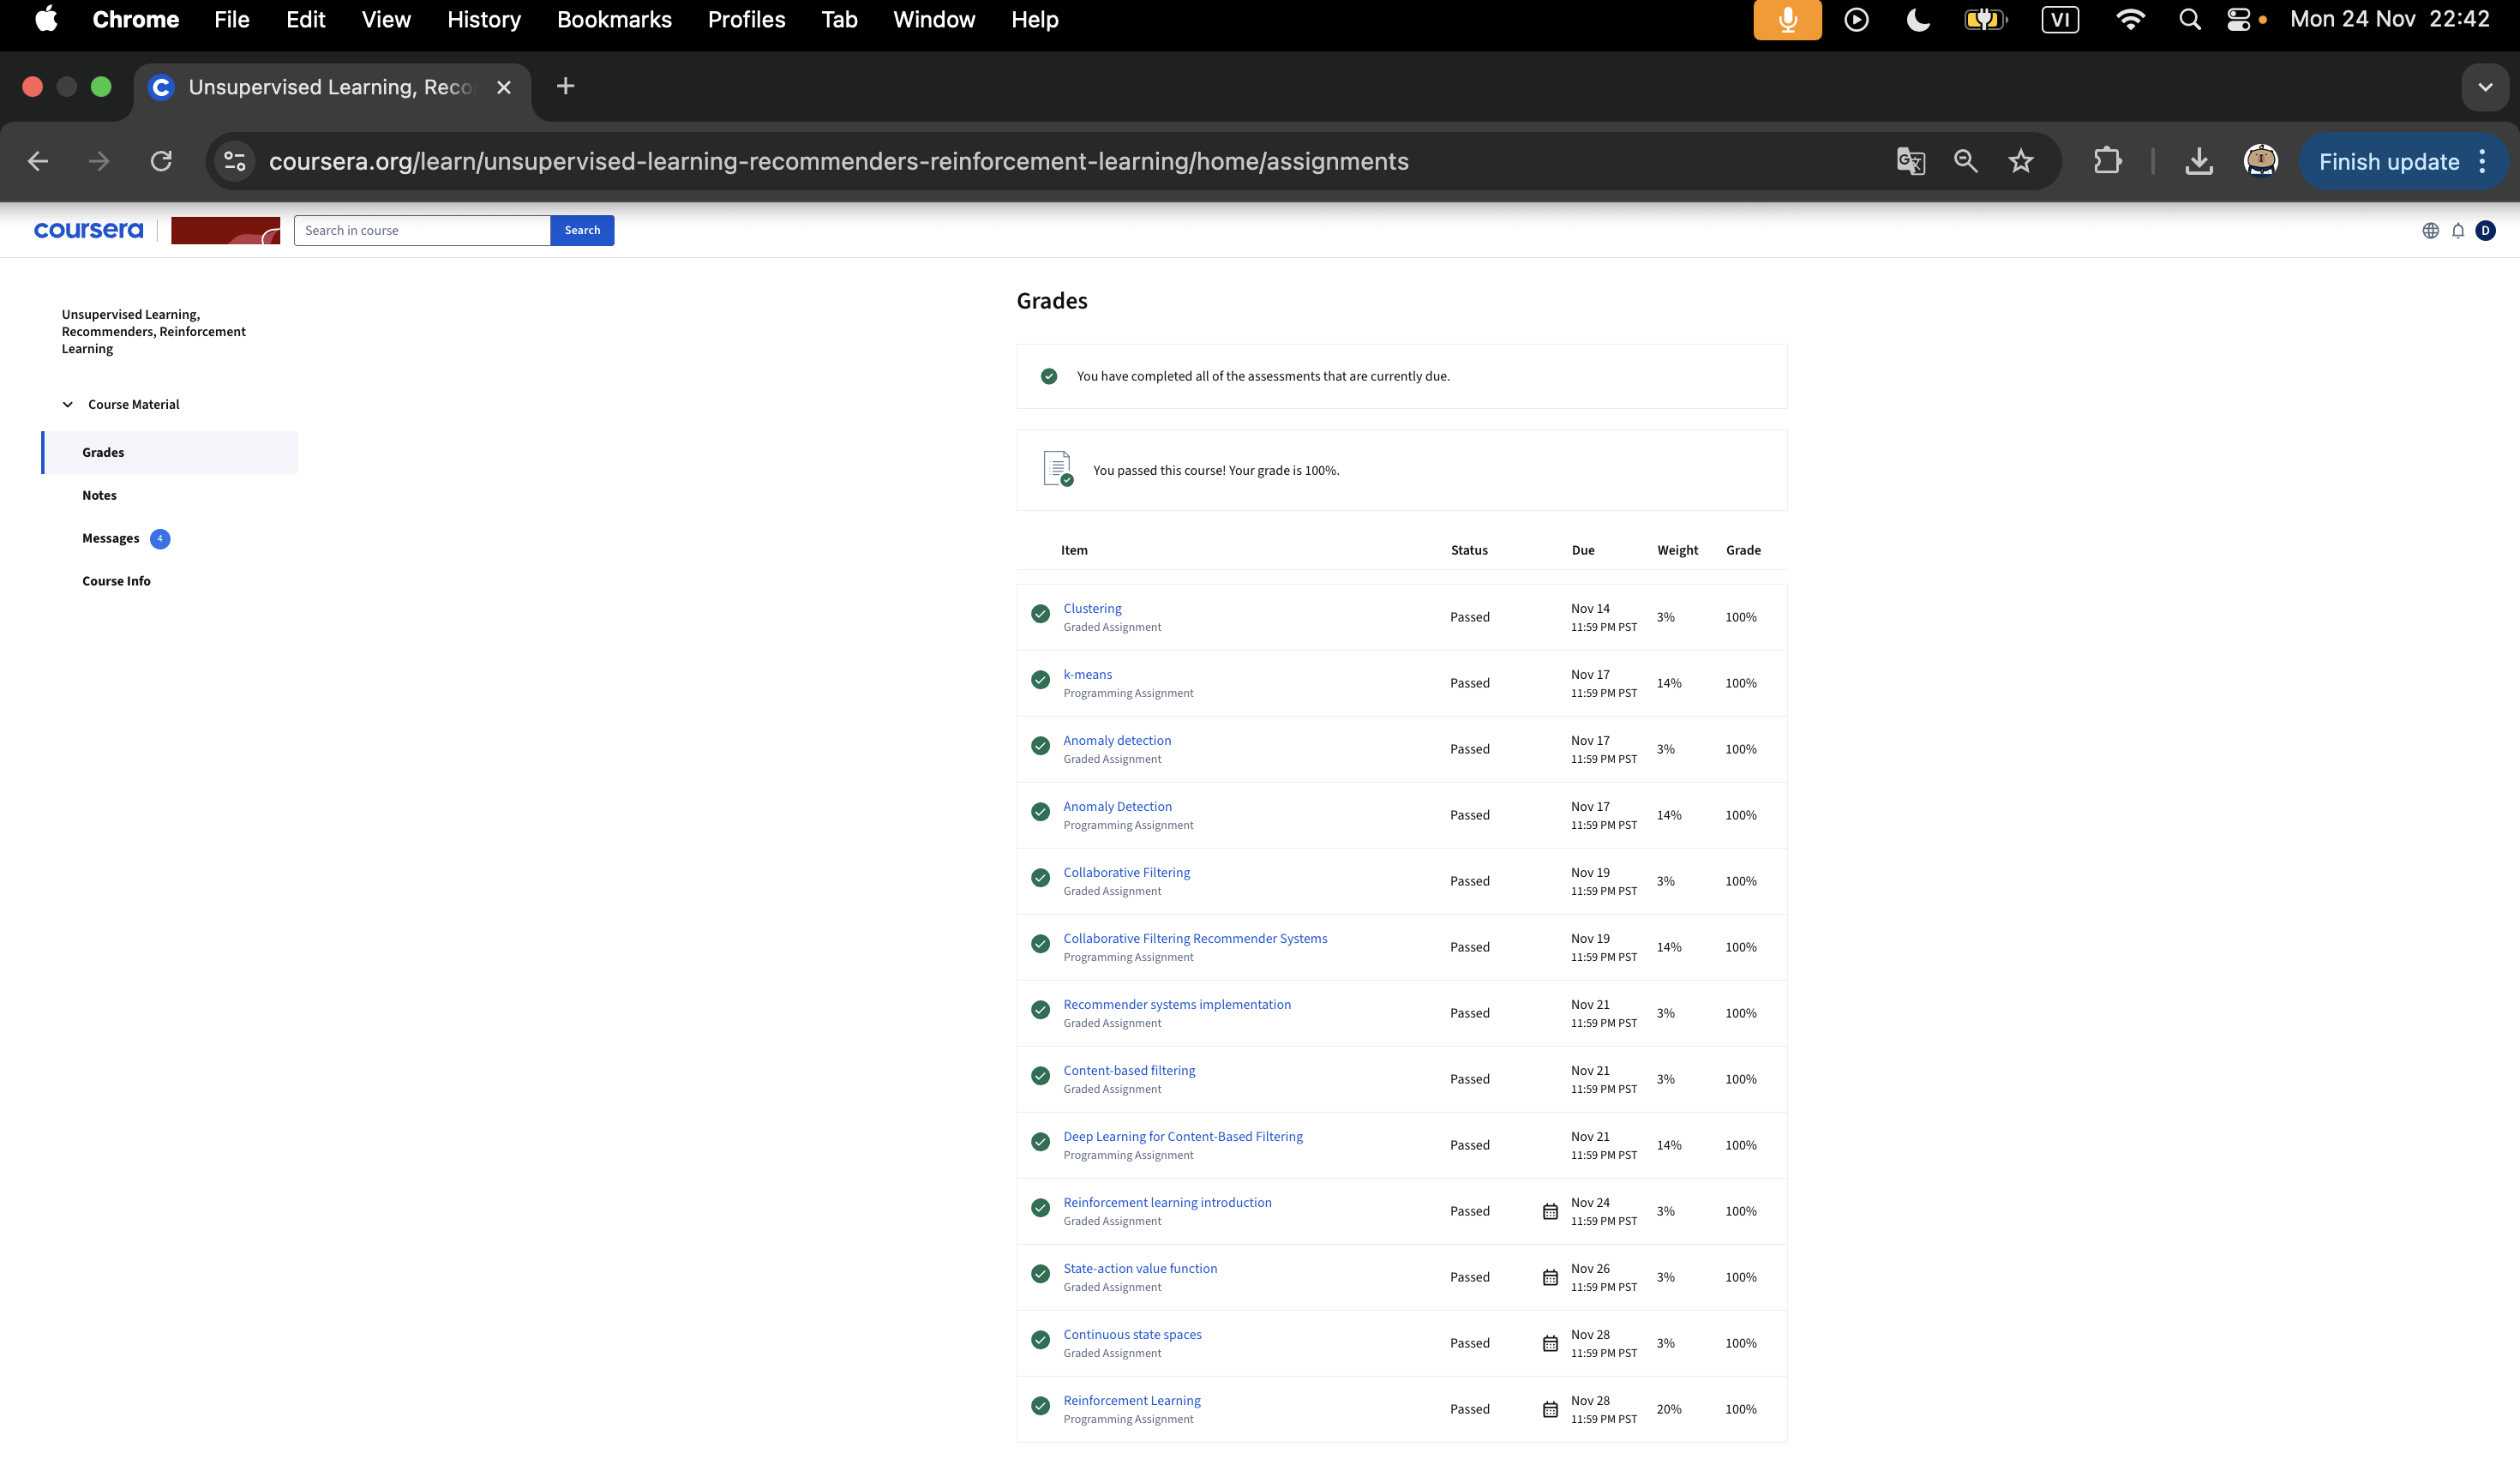
\includegraphics[scale=0.2]{Image/c3.png}
    \caption{Course 3 Completion Certificate}
\end{figure}

%----------------------------------------
\subsection{Week 1: Unsupervised Learning \& Anomaly Detection}
%----------------------------------------

\subsubsection{Key Insights and Learnings}

This module focused on algorithms that derive structure from data without pre-existing labels, essential for exploratory data analysis, pattern recognition, and system monitoring.

\begin{itemize}
    \item \textbf{Clustering with K-Means:} Learned to partition data into $k$ distinct groups by minimizing the variance within each cluster. 
    \begin{itemize}
        \item Applied the \textit{Elbow Method} to determine the optimal number of clusters ($k$) based on the distortion cost function.
        \item \textbf{Applications:} Market segmentation, document organization, and astronomical data analysis.
    \end{itemize}

    \item \textbf{Anomaly Detection:} Constructed probabilistic models using Gaussian (Normal) distribution to identify outliers or unusual events in a dataset.
    \begin{itemize}
        \item \textbf{Technique:} Estimating parameters ($\mu, \sigma^2$) to flag data points with very low probability density ($p(x) < \epsilon$).
        \item \textbf{Applications:} Fraud detection in finance, quality control in manufacturing, and server monitoring.
    \end{itemize}
    
    \item \textbf{Dimensionality Reduction (PCA):} Utilized \textbf{Principal Component Analysis} to compress data while retaining critical information. By finding underlying axes of maximum variance, PCA reduces feature dimensionality, which aids in data visualization (2D/3D) and improves the efficiency of supervised learning models.
\end{itemize}

\subsubsection{Learning Evidence}
\begin{figure}[H]
    \centering
    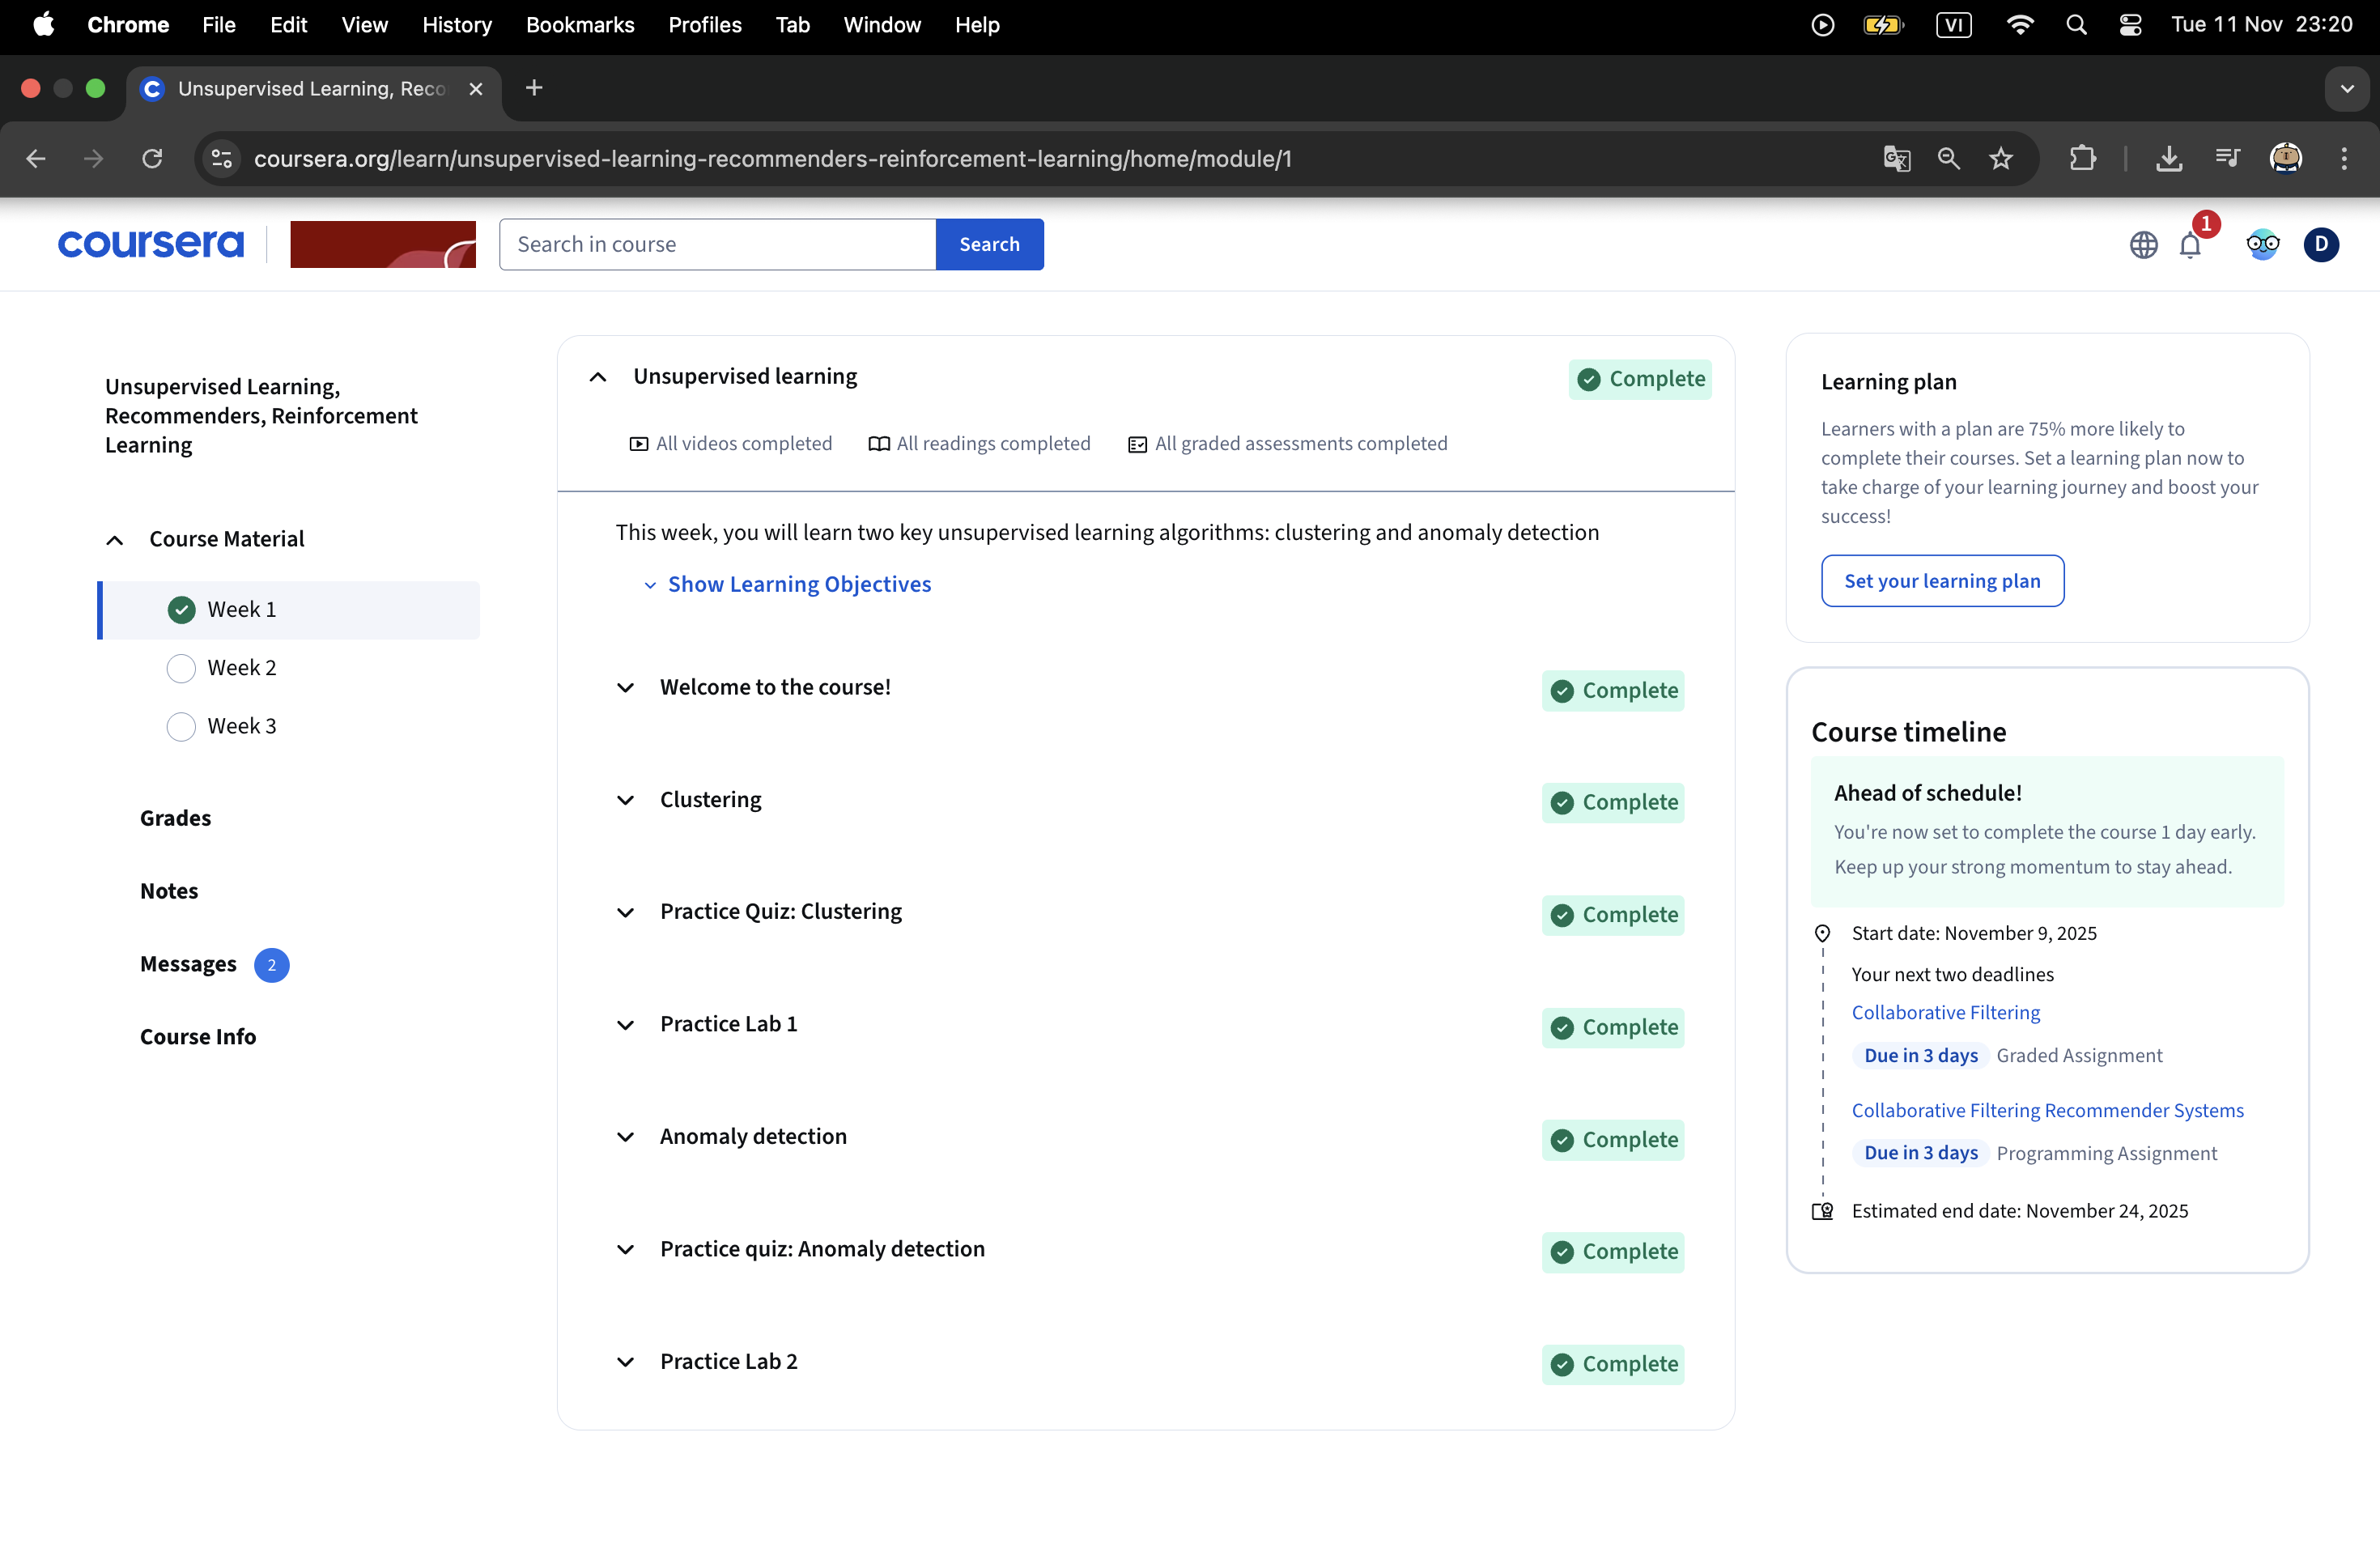
\includegraphics[scale=0.25]{Image/c3_w1.png}
    \caption{Lesson's completed date (11/11/2025)}
\end{figure}

\subsubsection{Graded Assignment Evidence}
\begin{figure}[H]
    \centering
    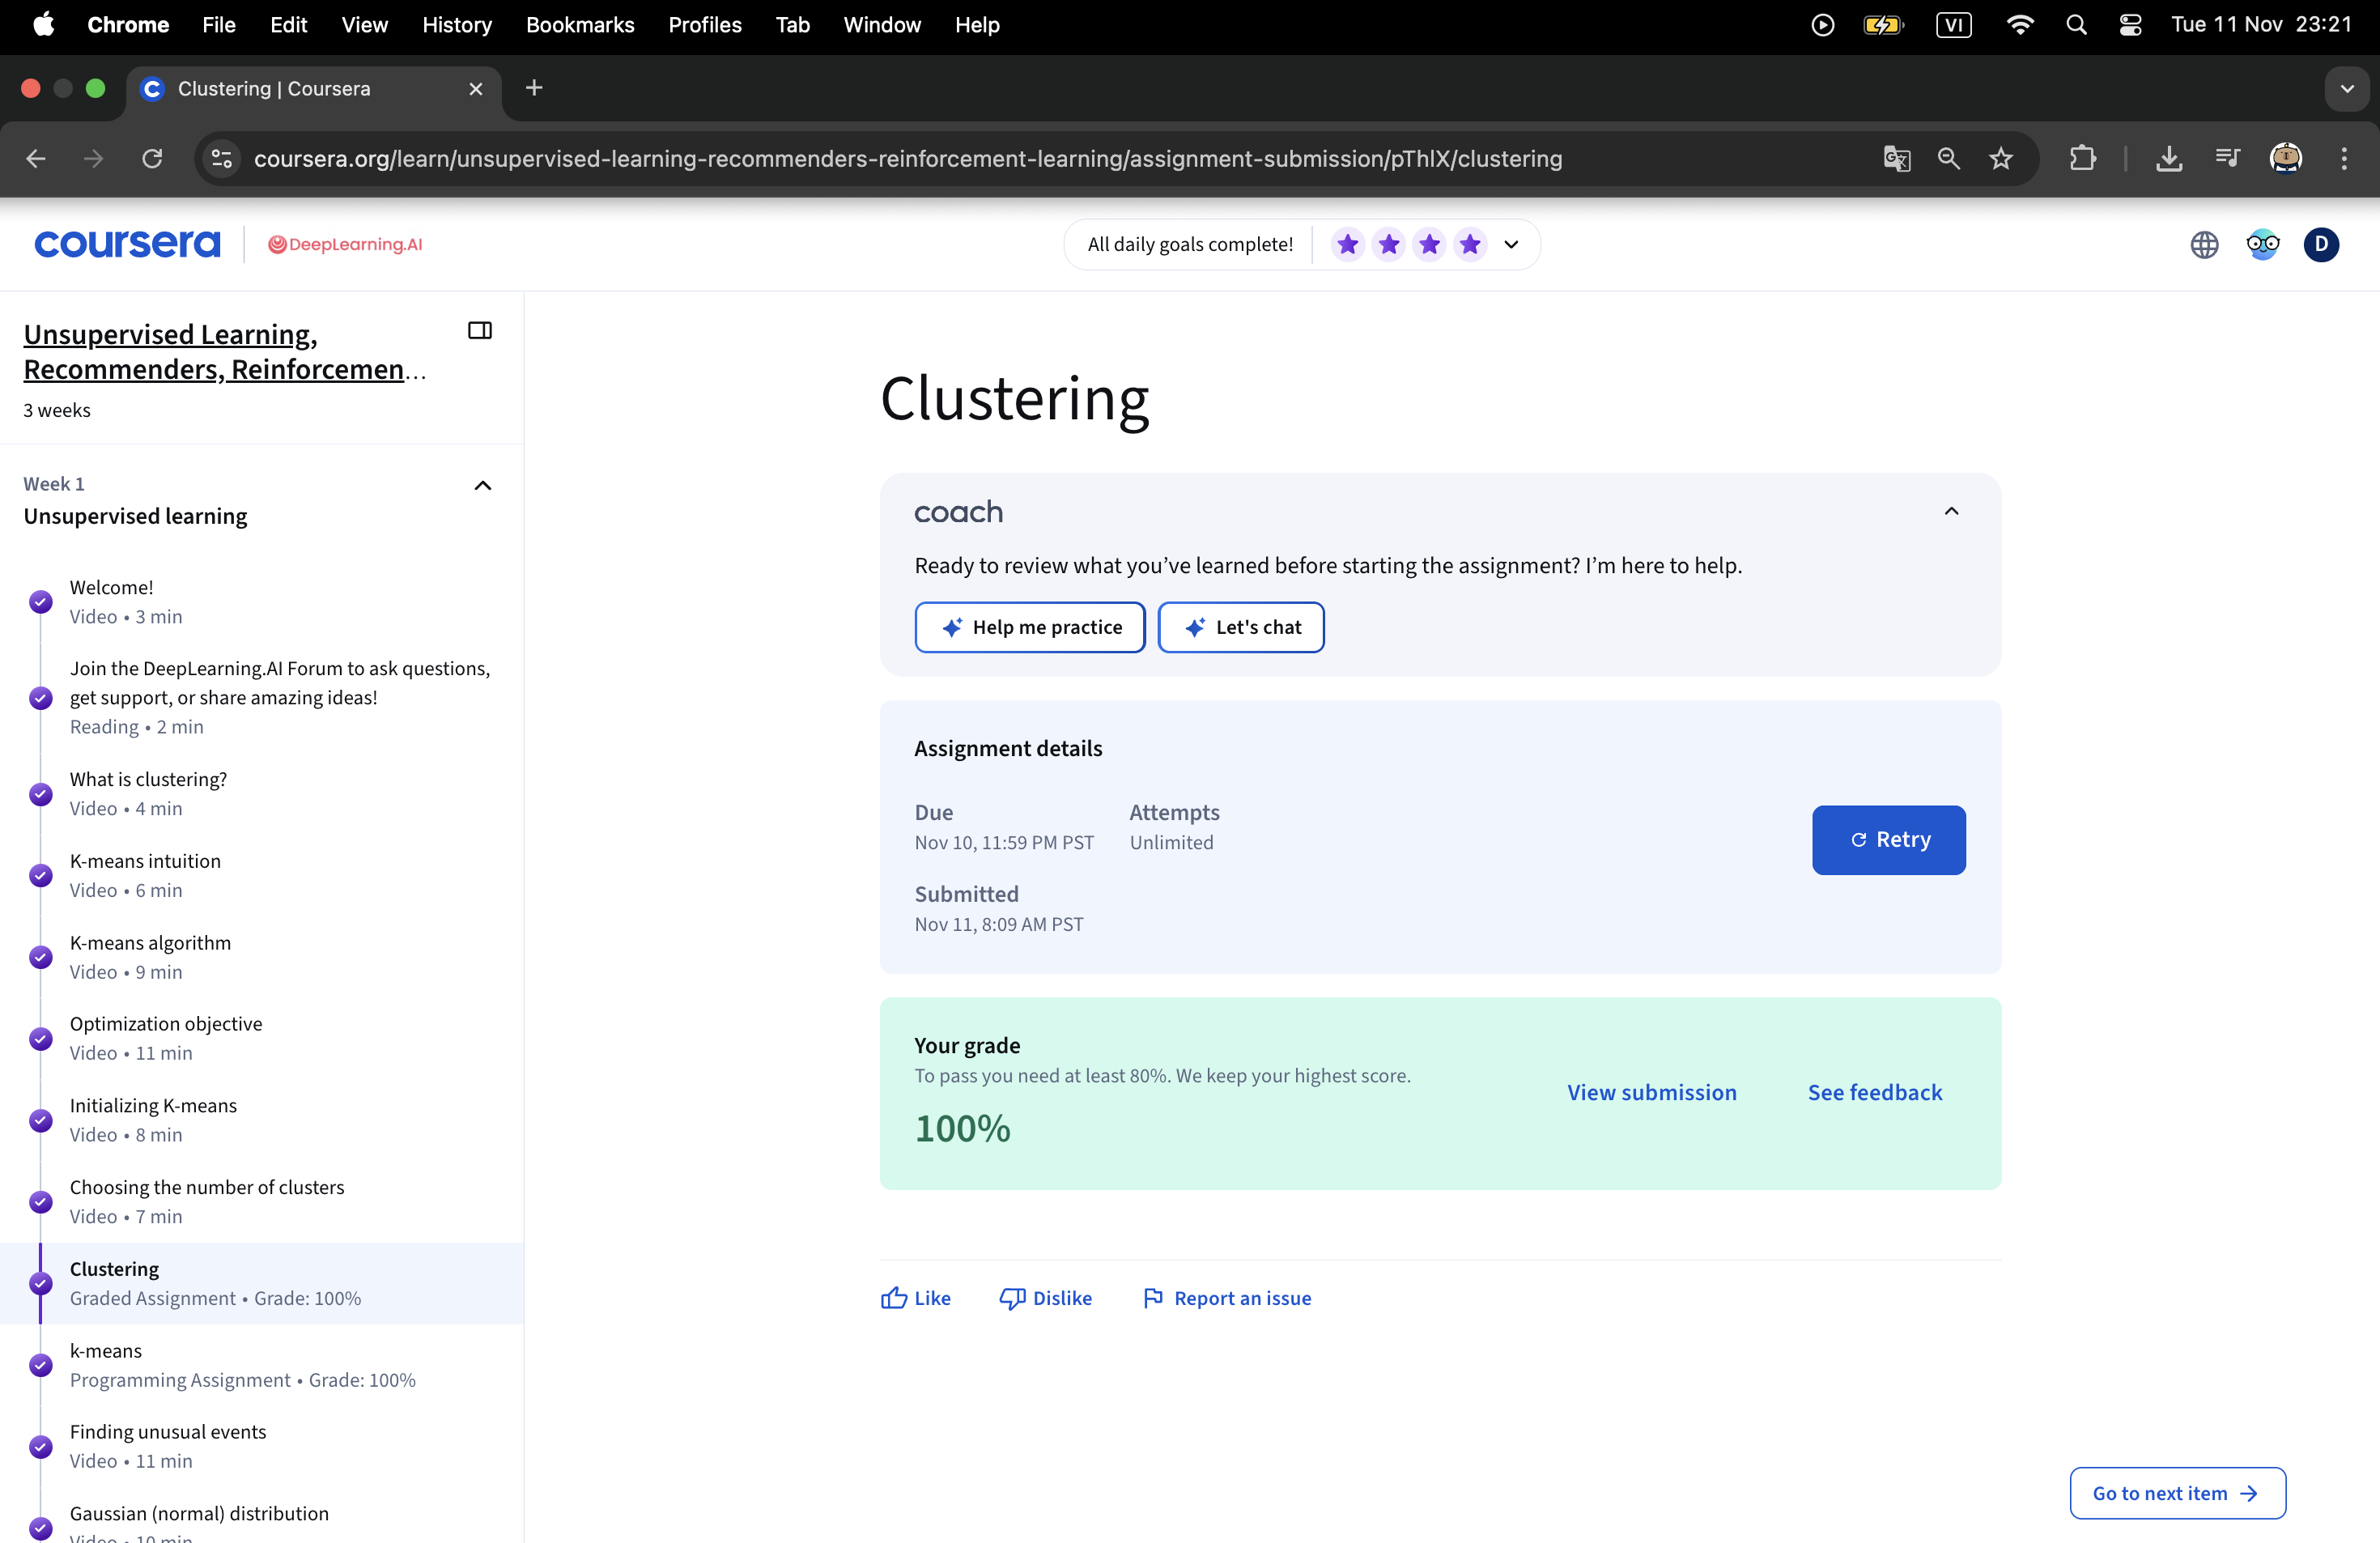
\includegraphics[scale=0.27]{Image/c3_w1_q1.png}
    \caption{Completed Graded Assignment 1 (Clustering)}
\end{figure}

\begin{figure}[H]
    \centering
    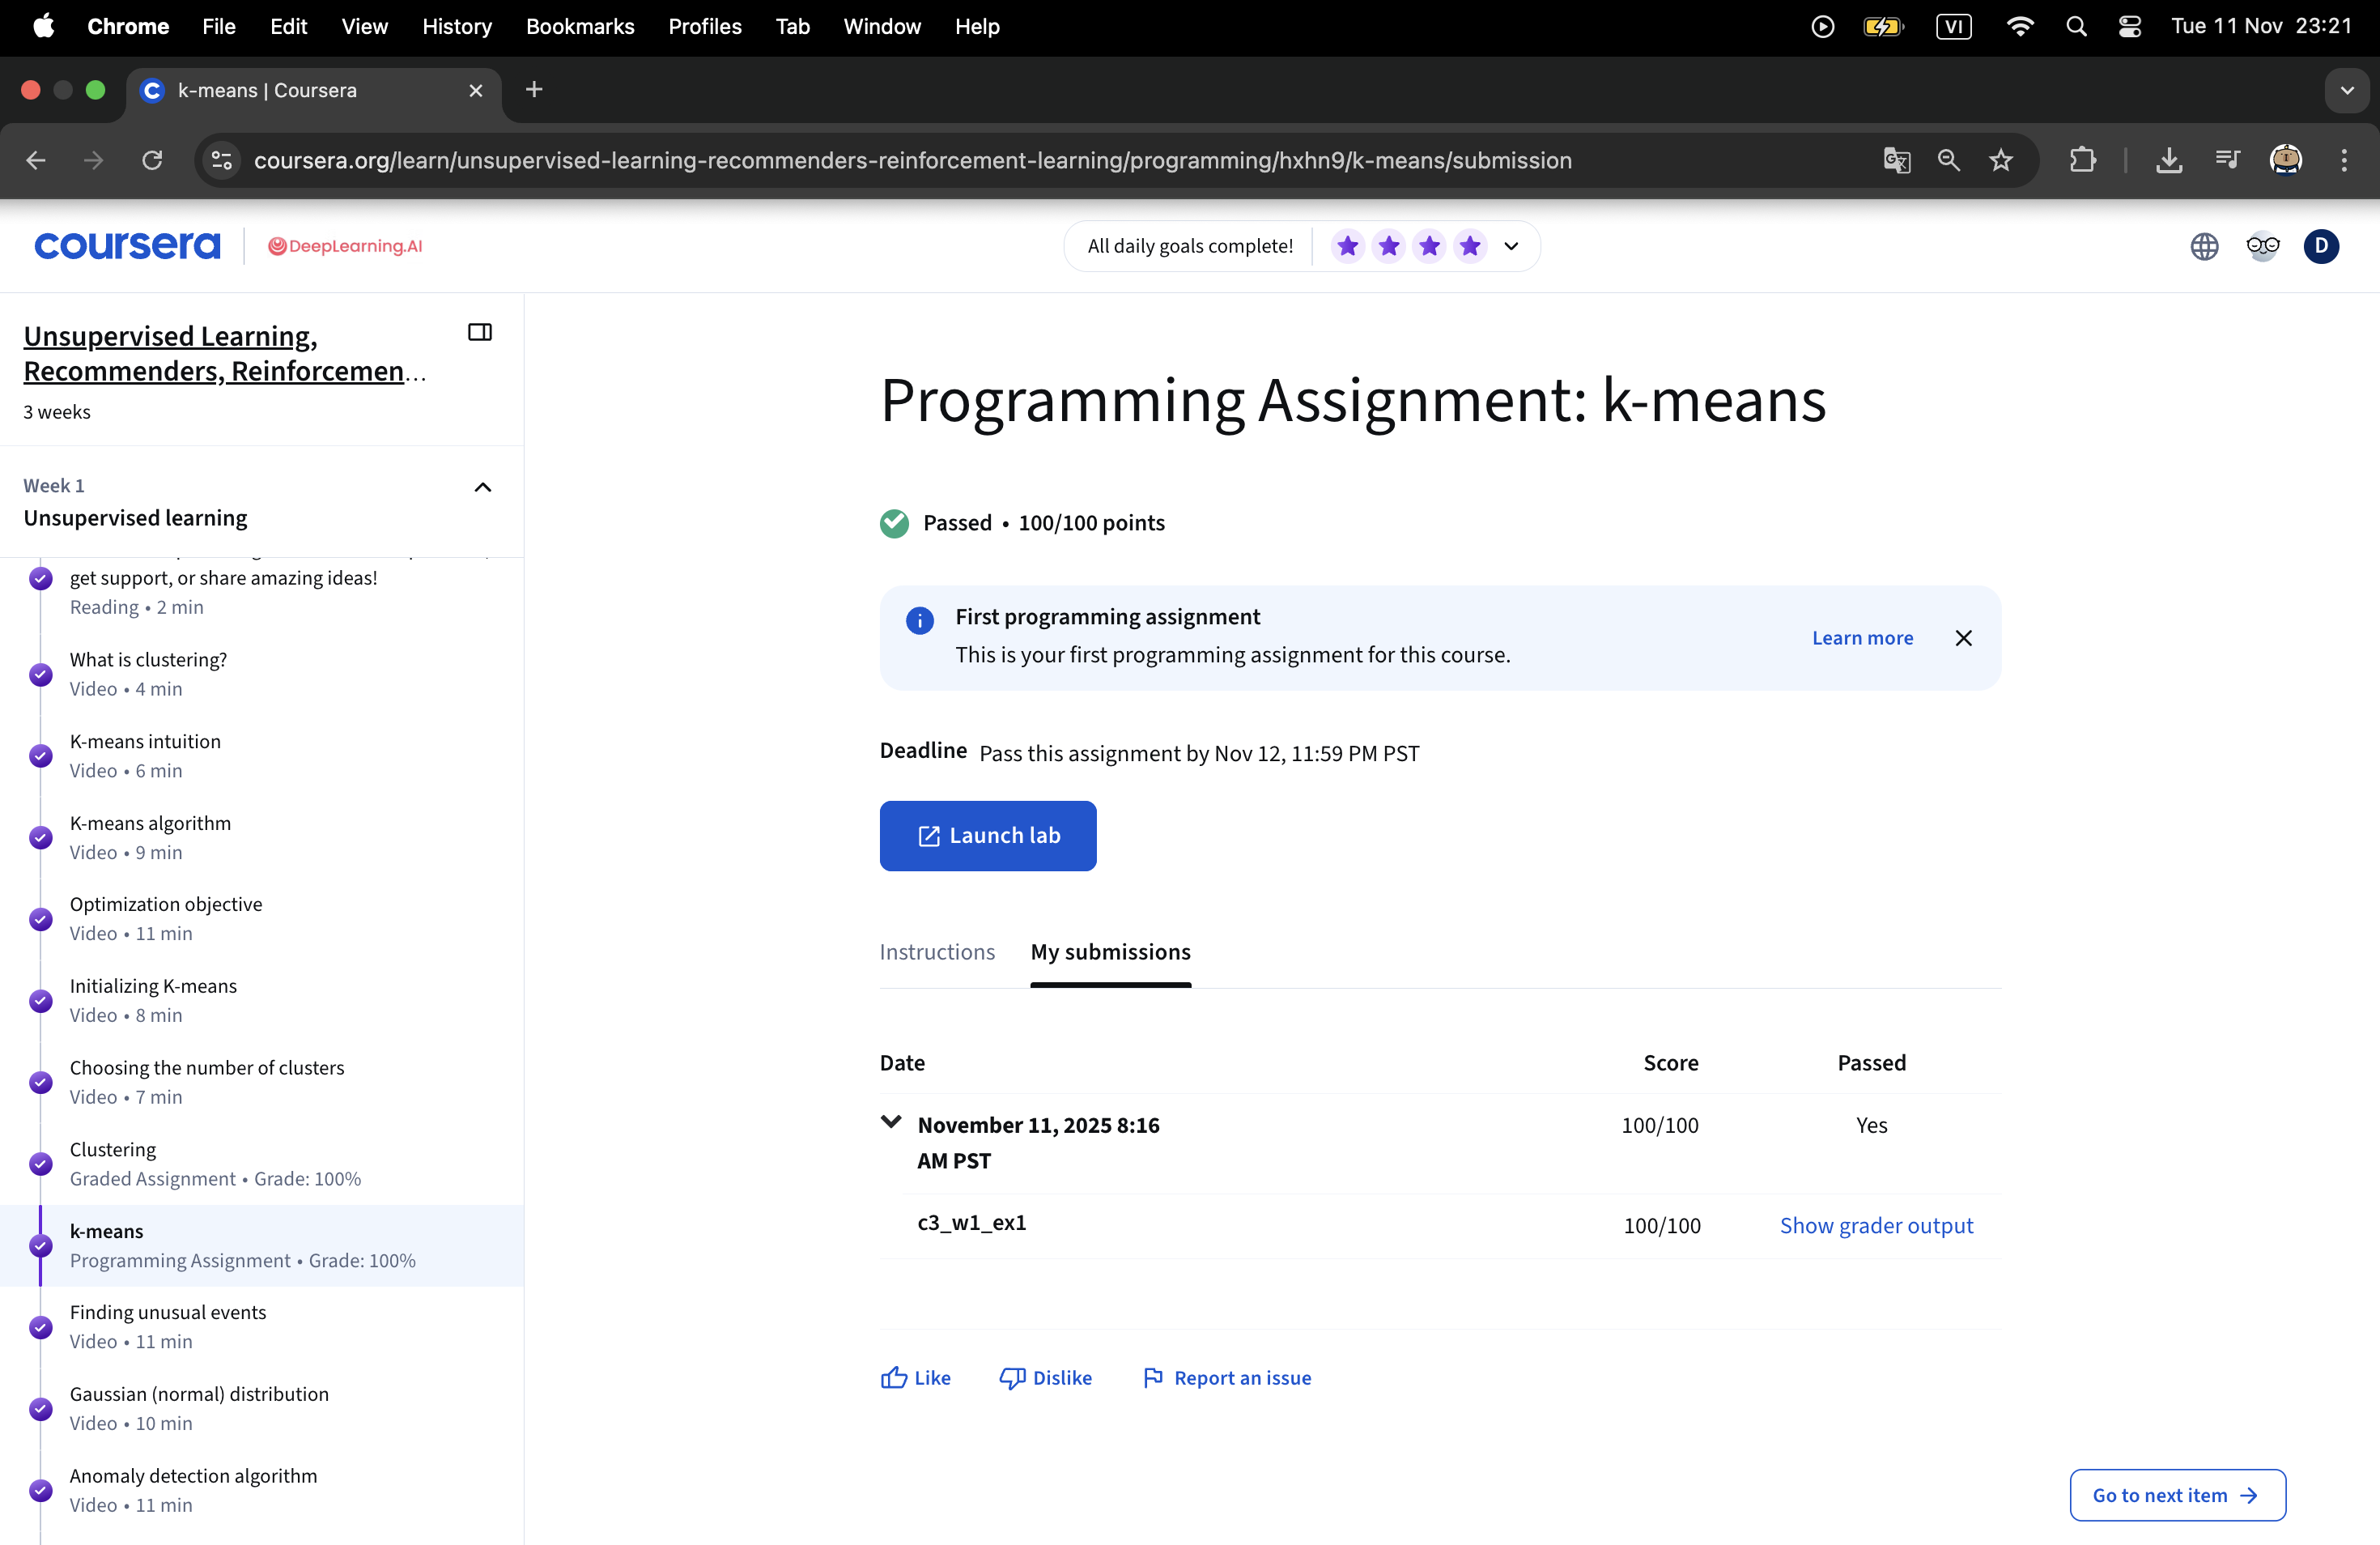
\includegraphics[scale=0.27]{Image/c3_w1_q2.png}
    \caption{Completed Programming Assignment (k-means)}
\end{figure}

\begin{figure}[H]
    \centering
    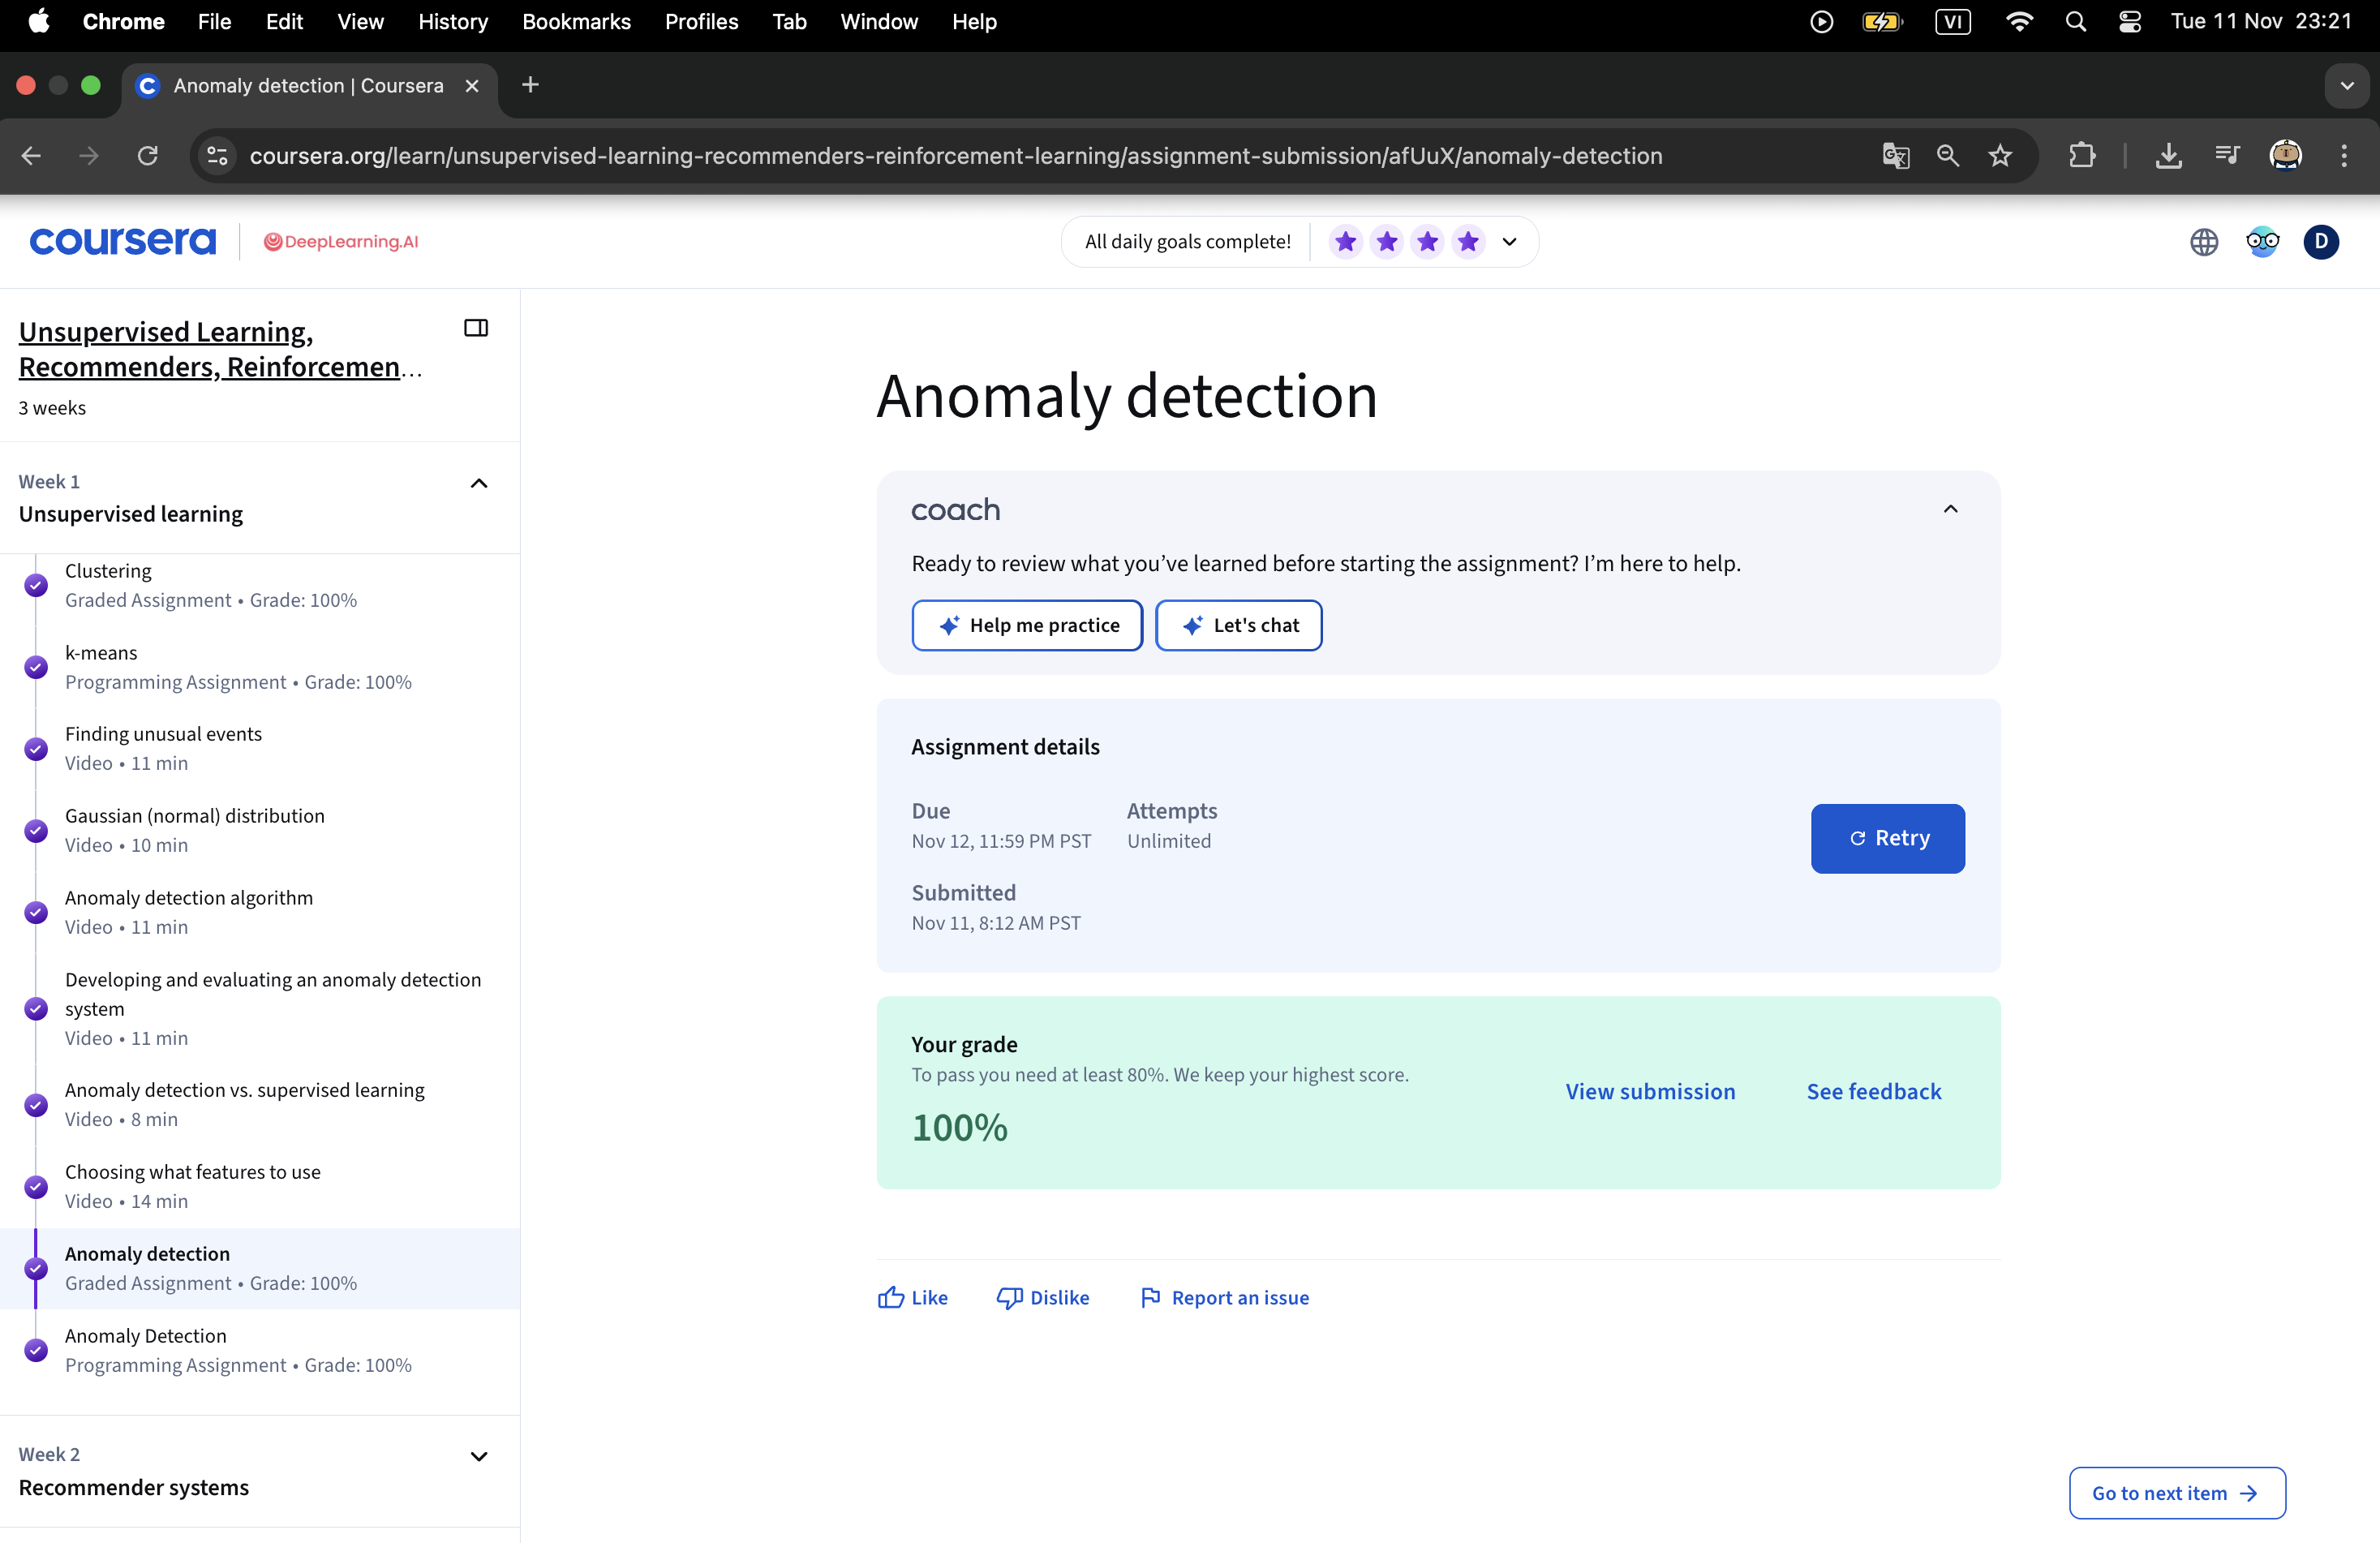
\includegraphics[scale=0.27]{Image/c3_w1_q3.png}
    \caption{Completed Graded Assignment 3 (Anomaly detection)}
\end{figure}


\begin{figure}[H]
    \centering
    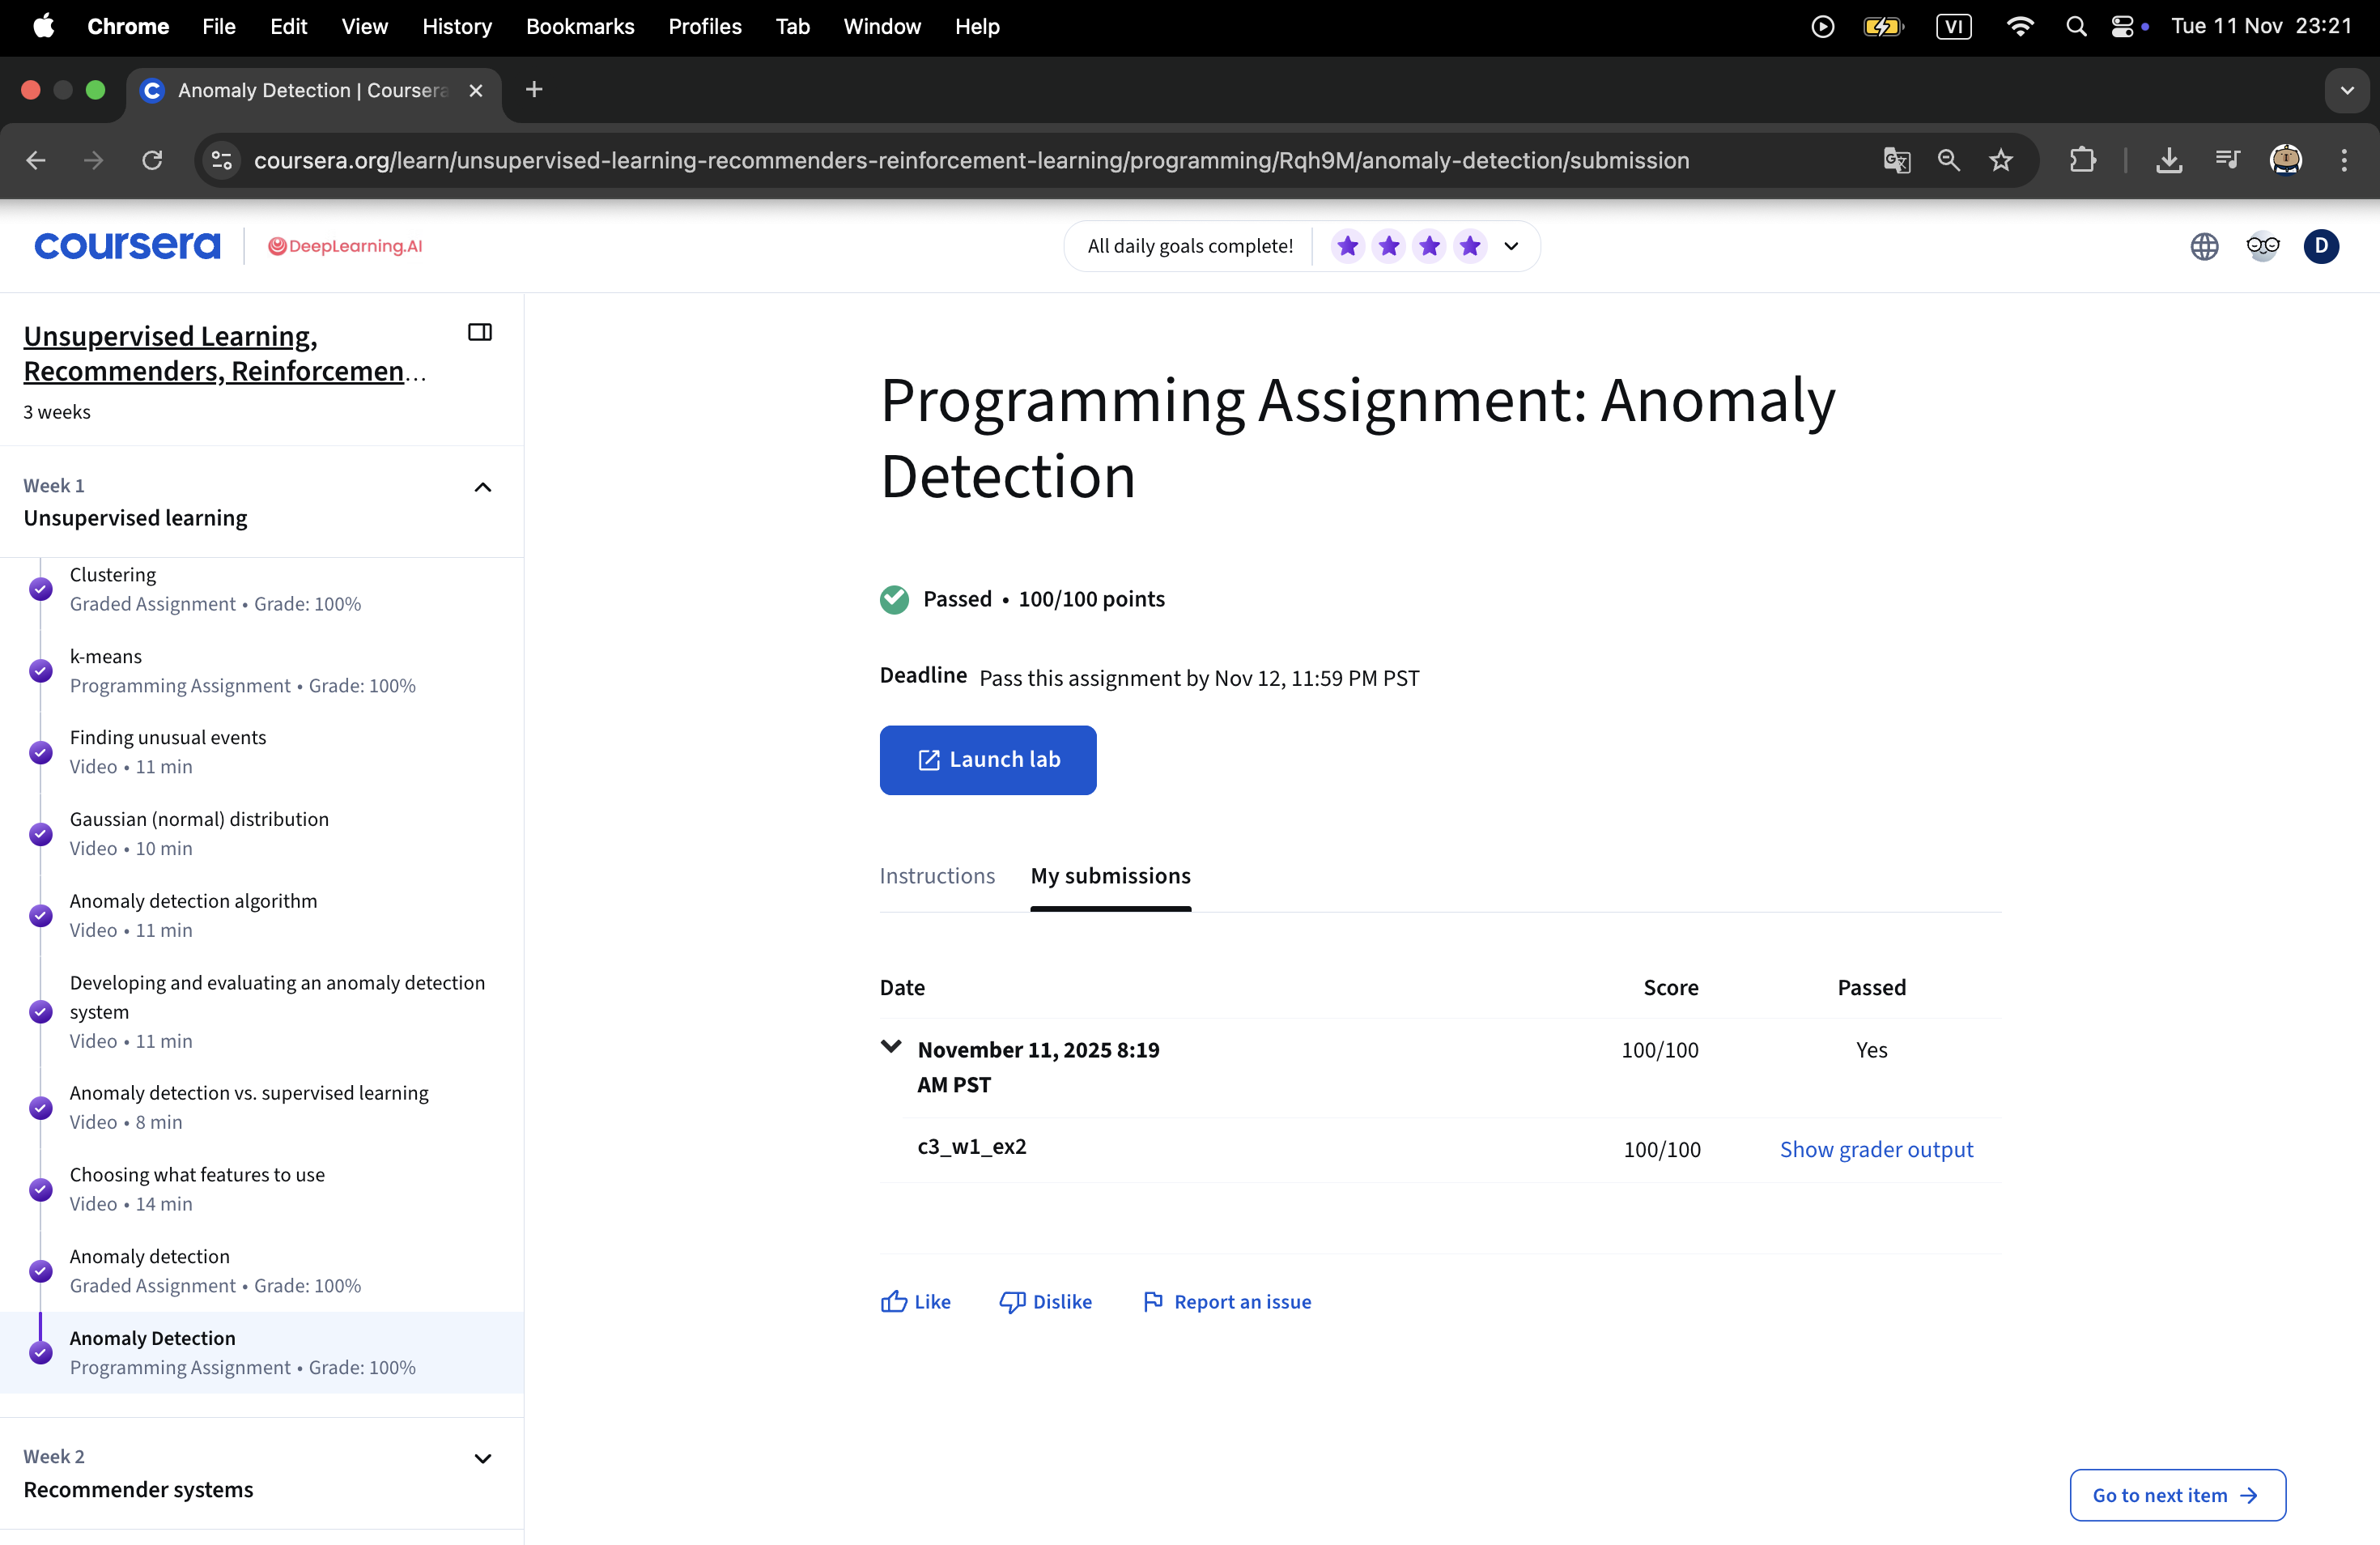
\includegraphics[scale=0.27]{Image/c3_w1_q4.png}
    \caption{Completed Programming Assignment (Anomaly Detection)}
\end{figure}

%----------------------------------------
\subsection{Week 2: Recommender Systems}
%----------------------------------------

\subsubsection{Key Insights and Learnings}

This module demystified the architecture behind modern personalization engines used by platforms like Netflix and Amazon, implementing both content-based and interaction-based approaches.

\begin{itemize}
    \item \textbf{Collaborative Filtering:} Implemented algorithms that predict user preferences based on community behavior. The model learns that users who agreed in the past will likely agree in the future, without needing explicit item attributes.
    
    \item \textbf{Content-Based Filtering:} Developed models that recommend items based on the similarity between item features (e.g., genre, keywords) and a user's profile.
    
    \item \textbf{Matrix Factorization \& Embeddings:} 
    \begin{itemize}
        \item Learned to represent users and items as vectors in a lower-dimensional space.
        \item The dot product of these vectors predicts the user rating ($y^{(i,j)} = w^{(j)} \cdot x^{(i)} + b$).
        \item Utilized \textbf{Mean Normalization} to handle the "Cold Start" problem for new users with no history.
    \end{itemize}
\end{itemize}

\subsubsection{Learning Evidence}
\begin{figure}[H]
    \centering
    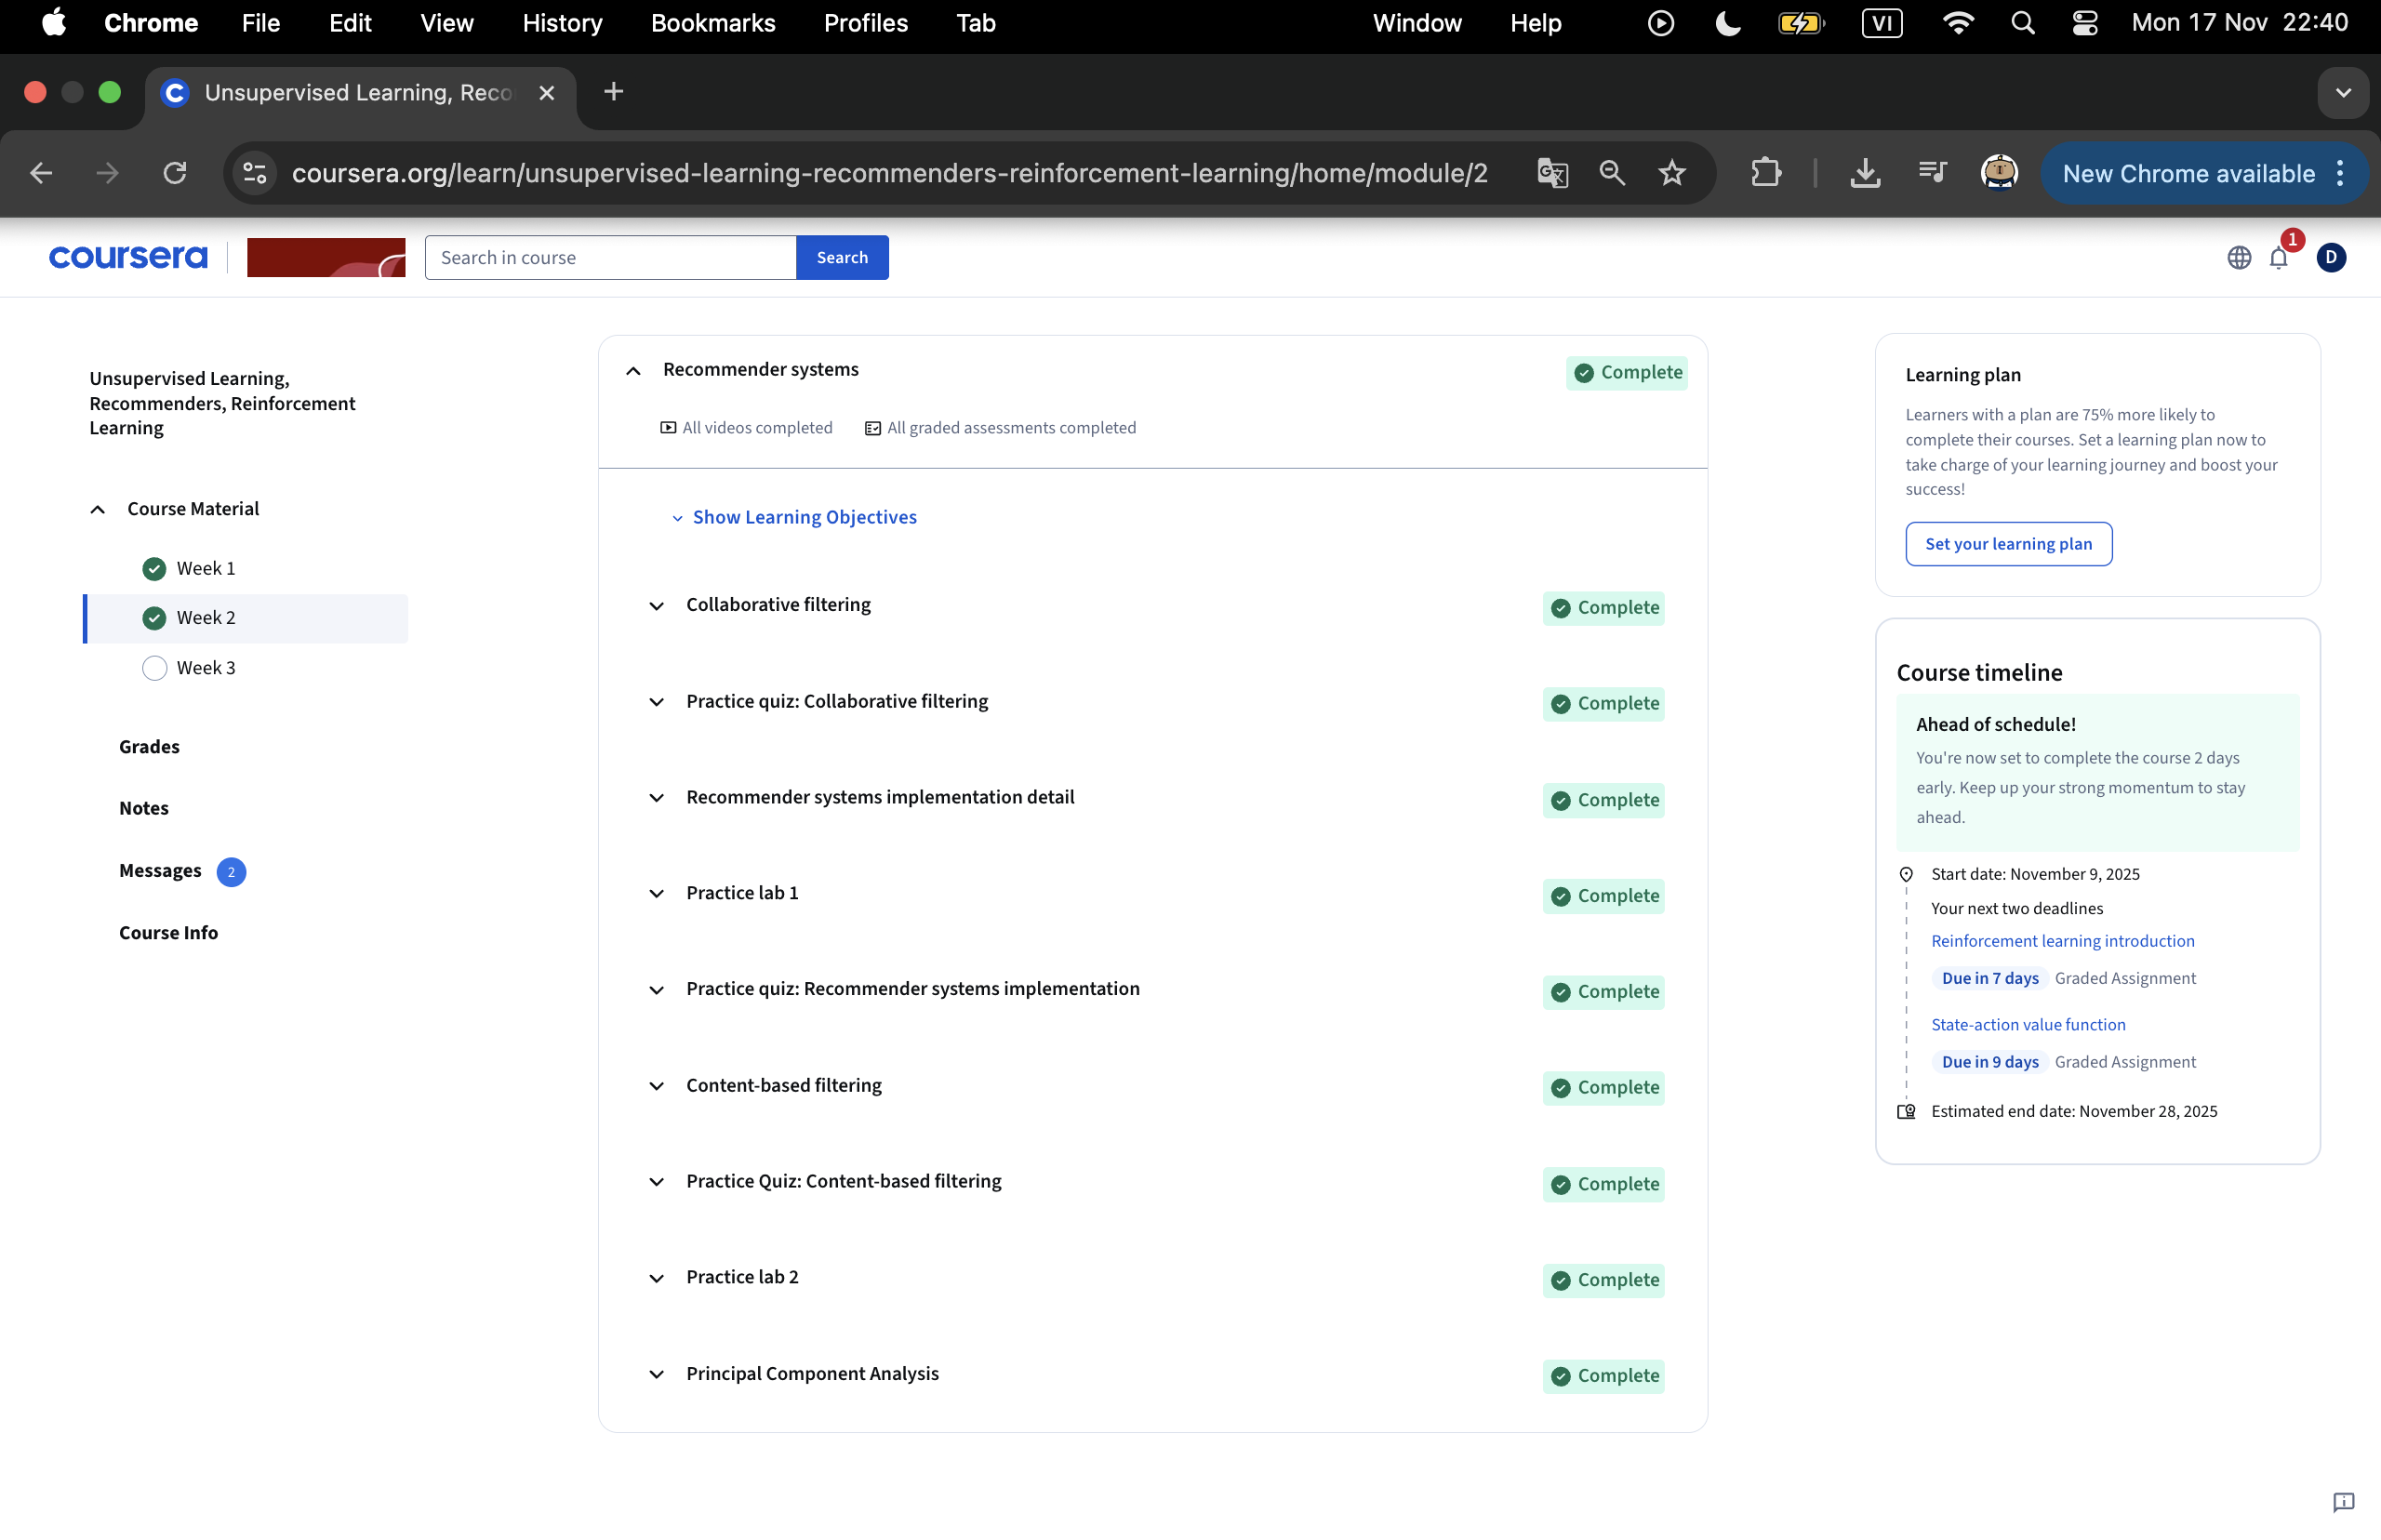
\includegraphics[scale=0.35]{Image/c3_w2.png}
    \caption{Lesson's completed date (17/11/2025)}
\end{figure}

\subsubsection{Graded Assignment Evidence}
\begin{figure}[H]
    \centering
    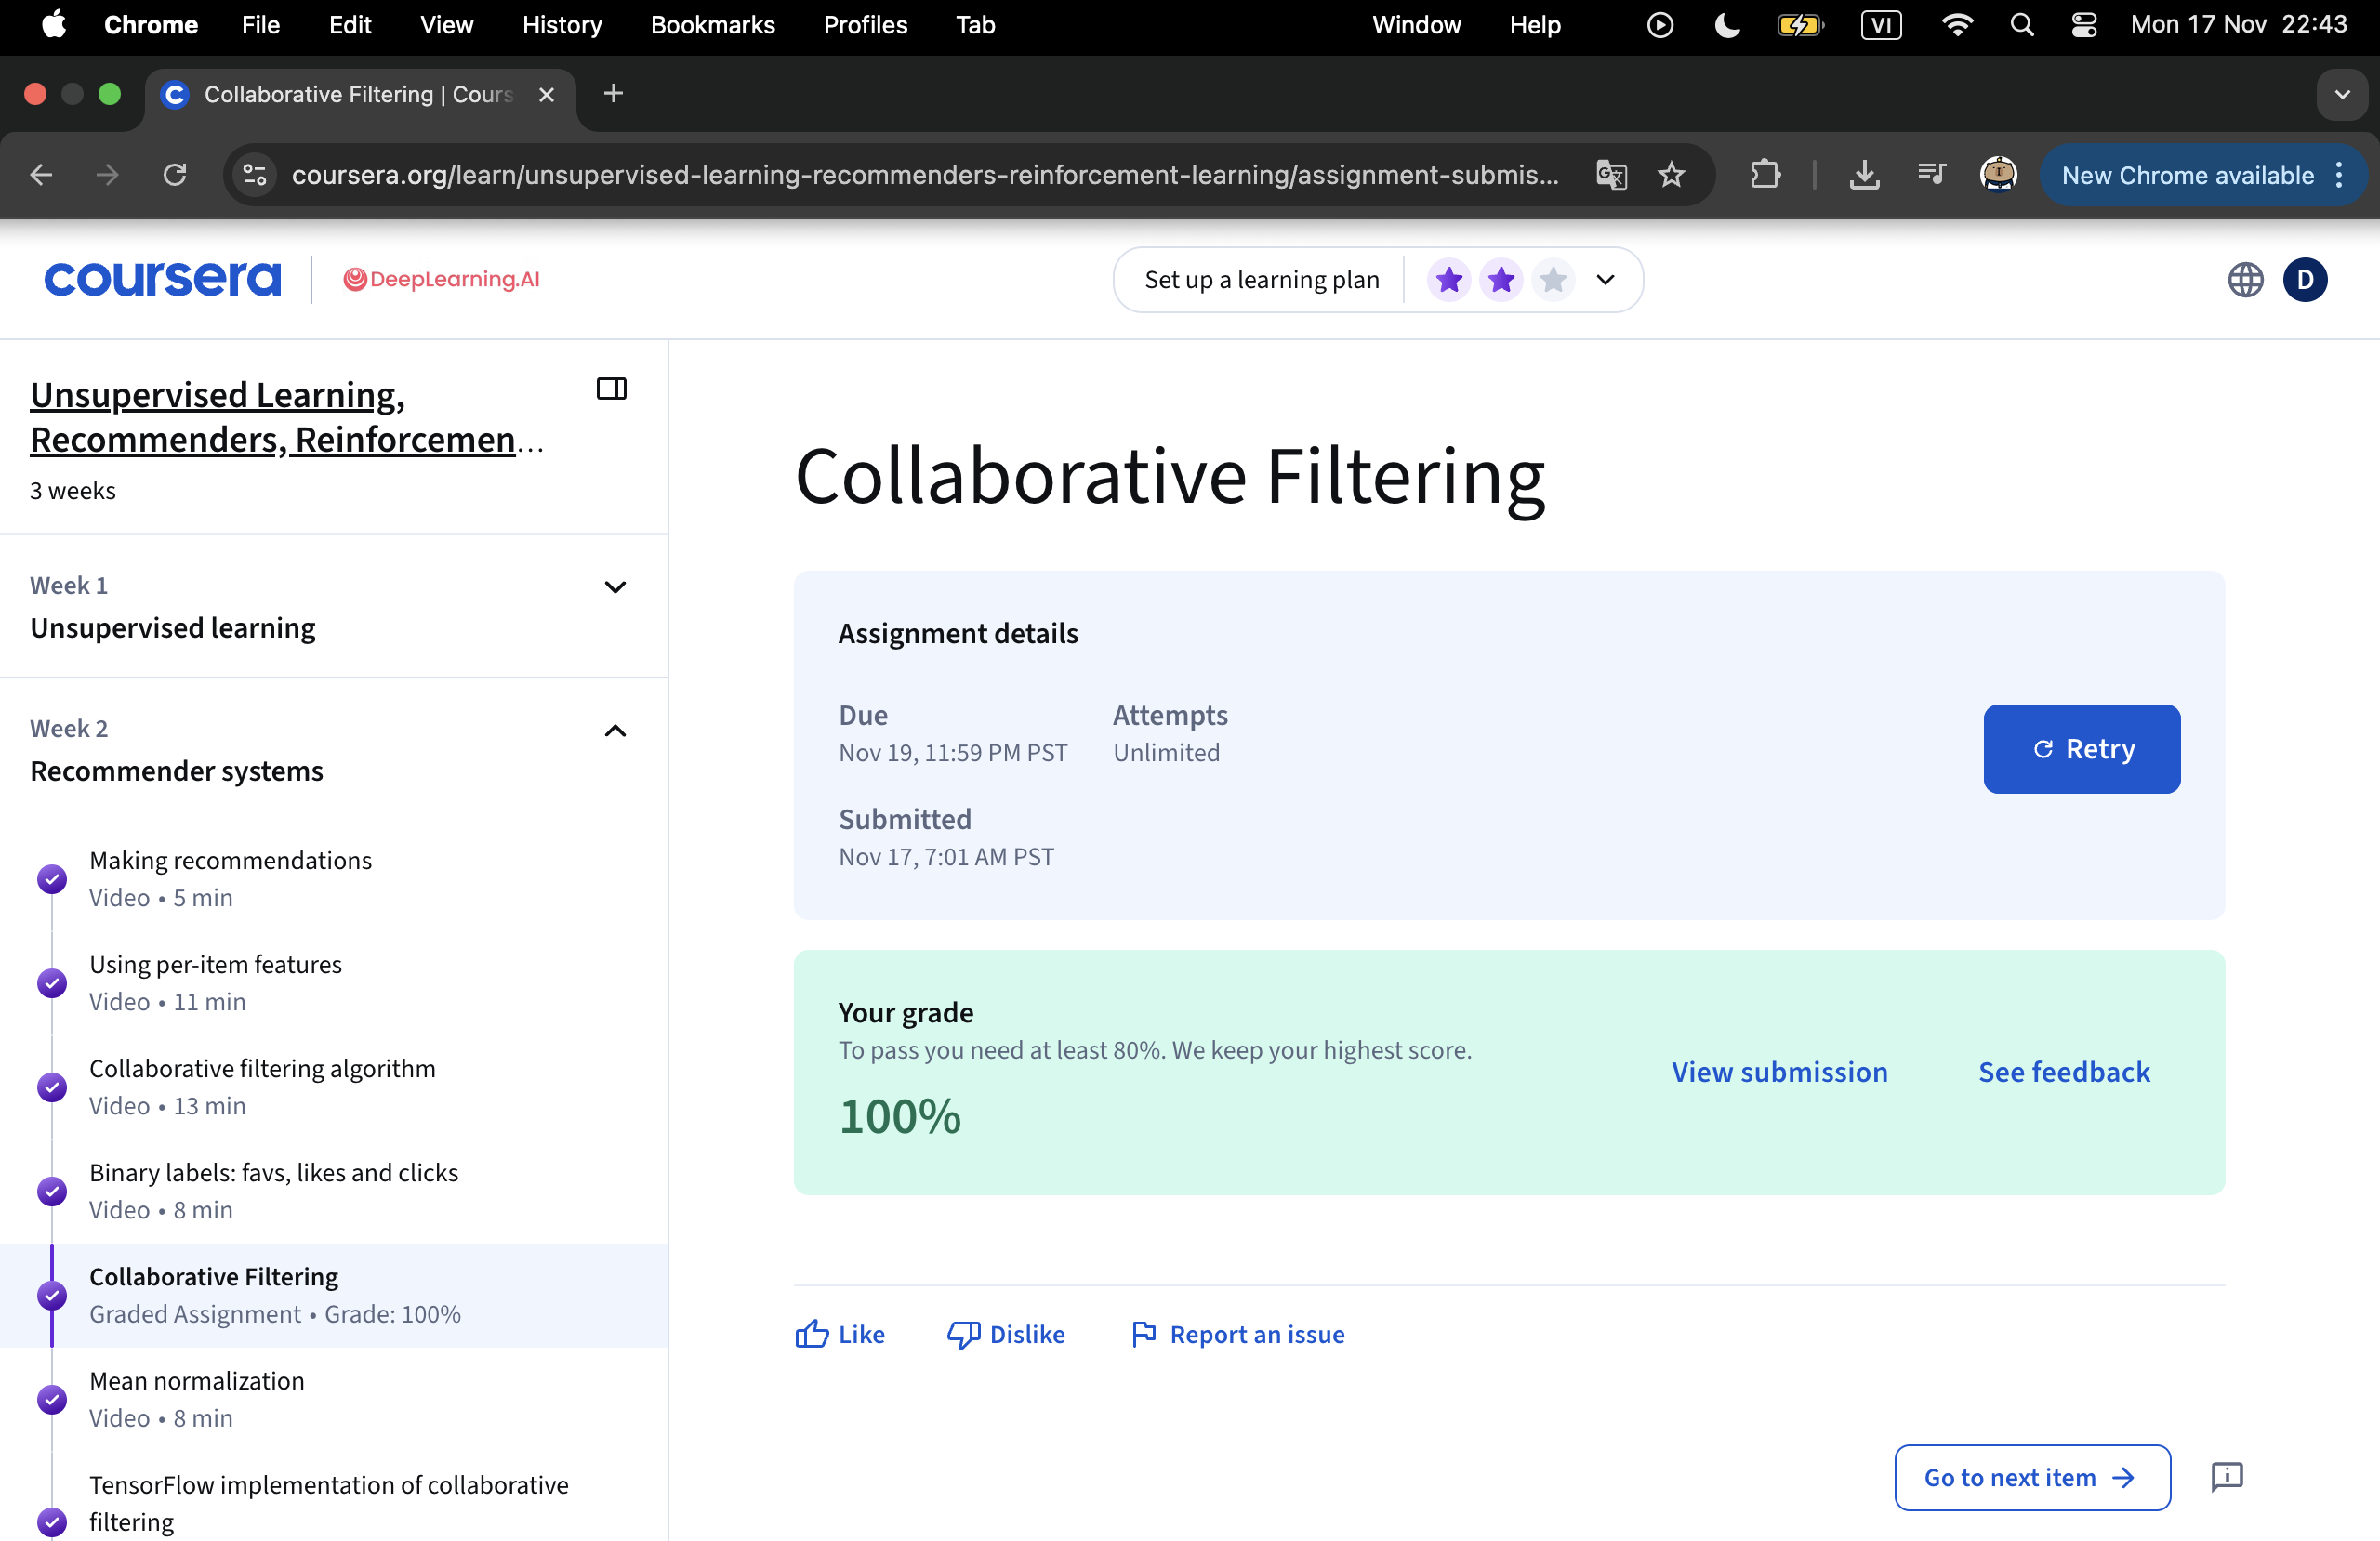
\includegraphics[scale=0.27]{Image/c3_w2_q1.png}
    \caption{Completed Graded Assignment 1 (Collaborative Filtering)}
\end{figure}

\begin{figure}[H]
    \centering
    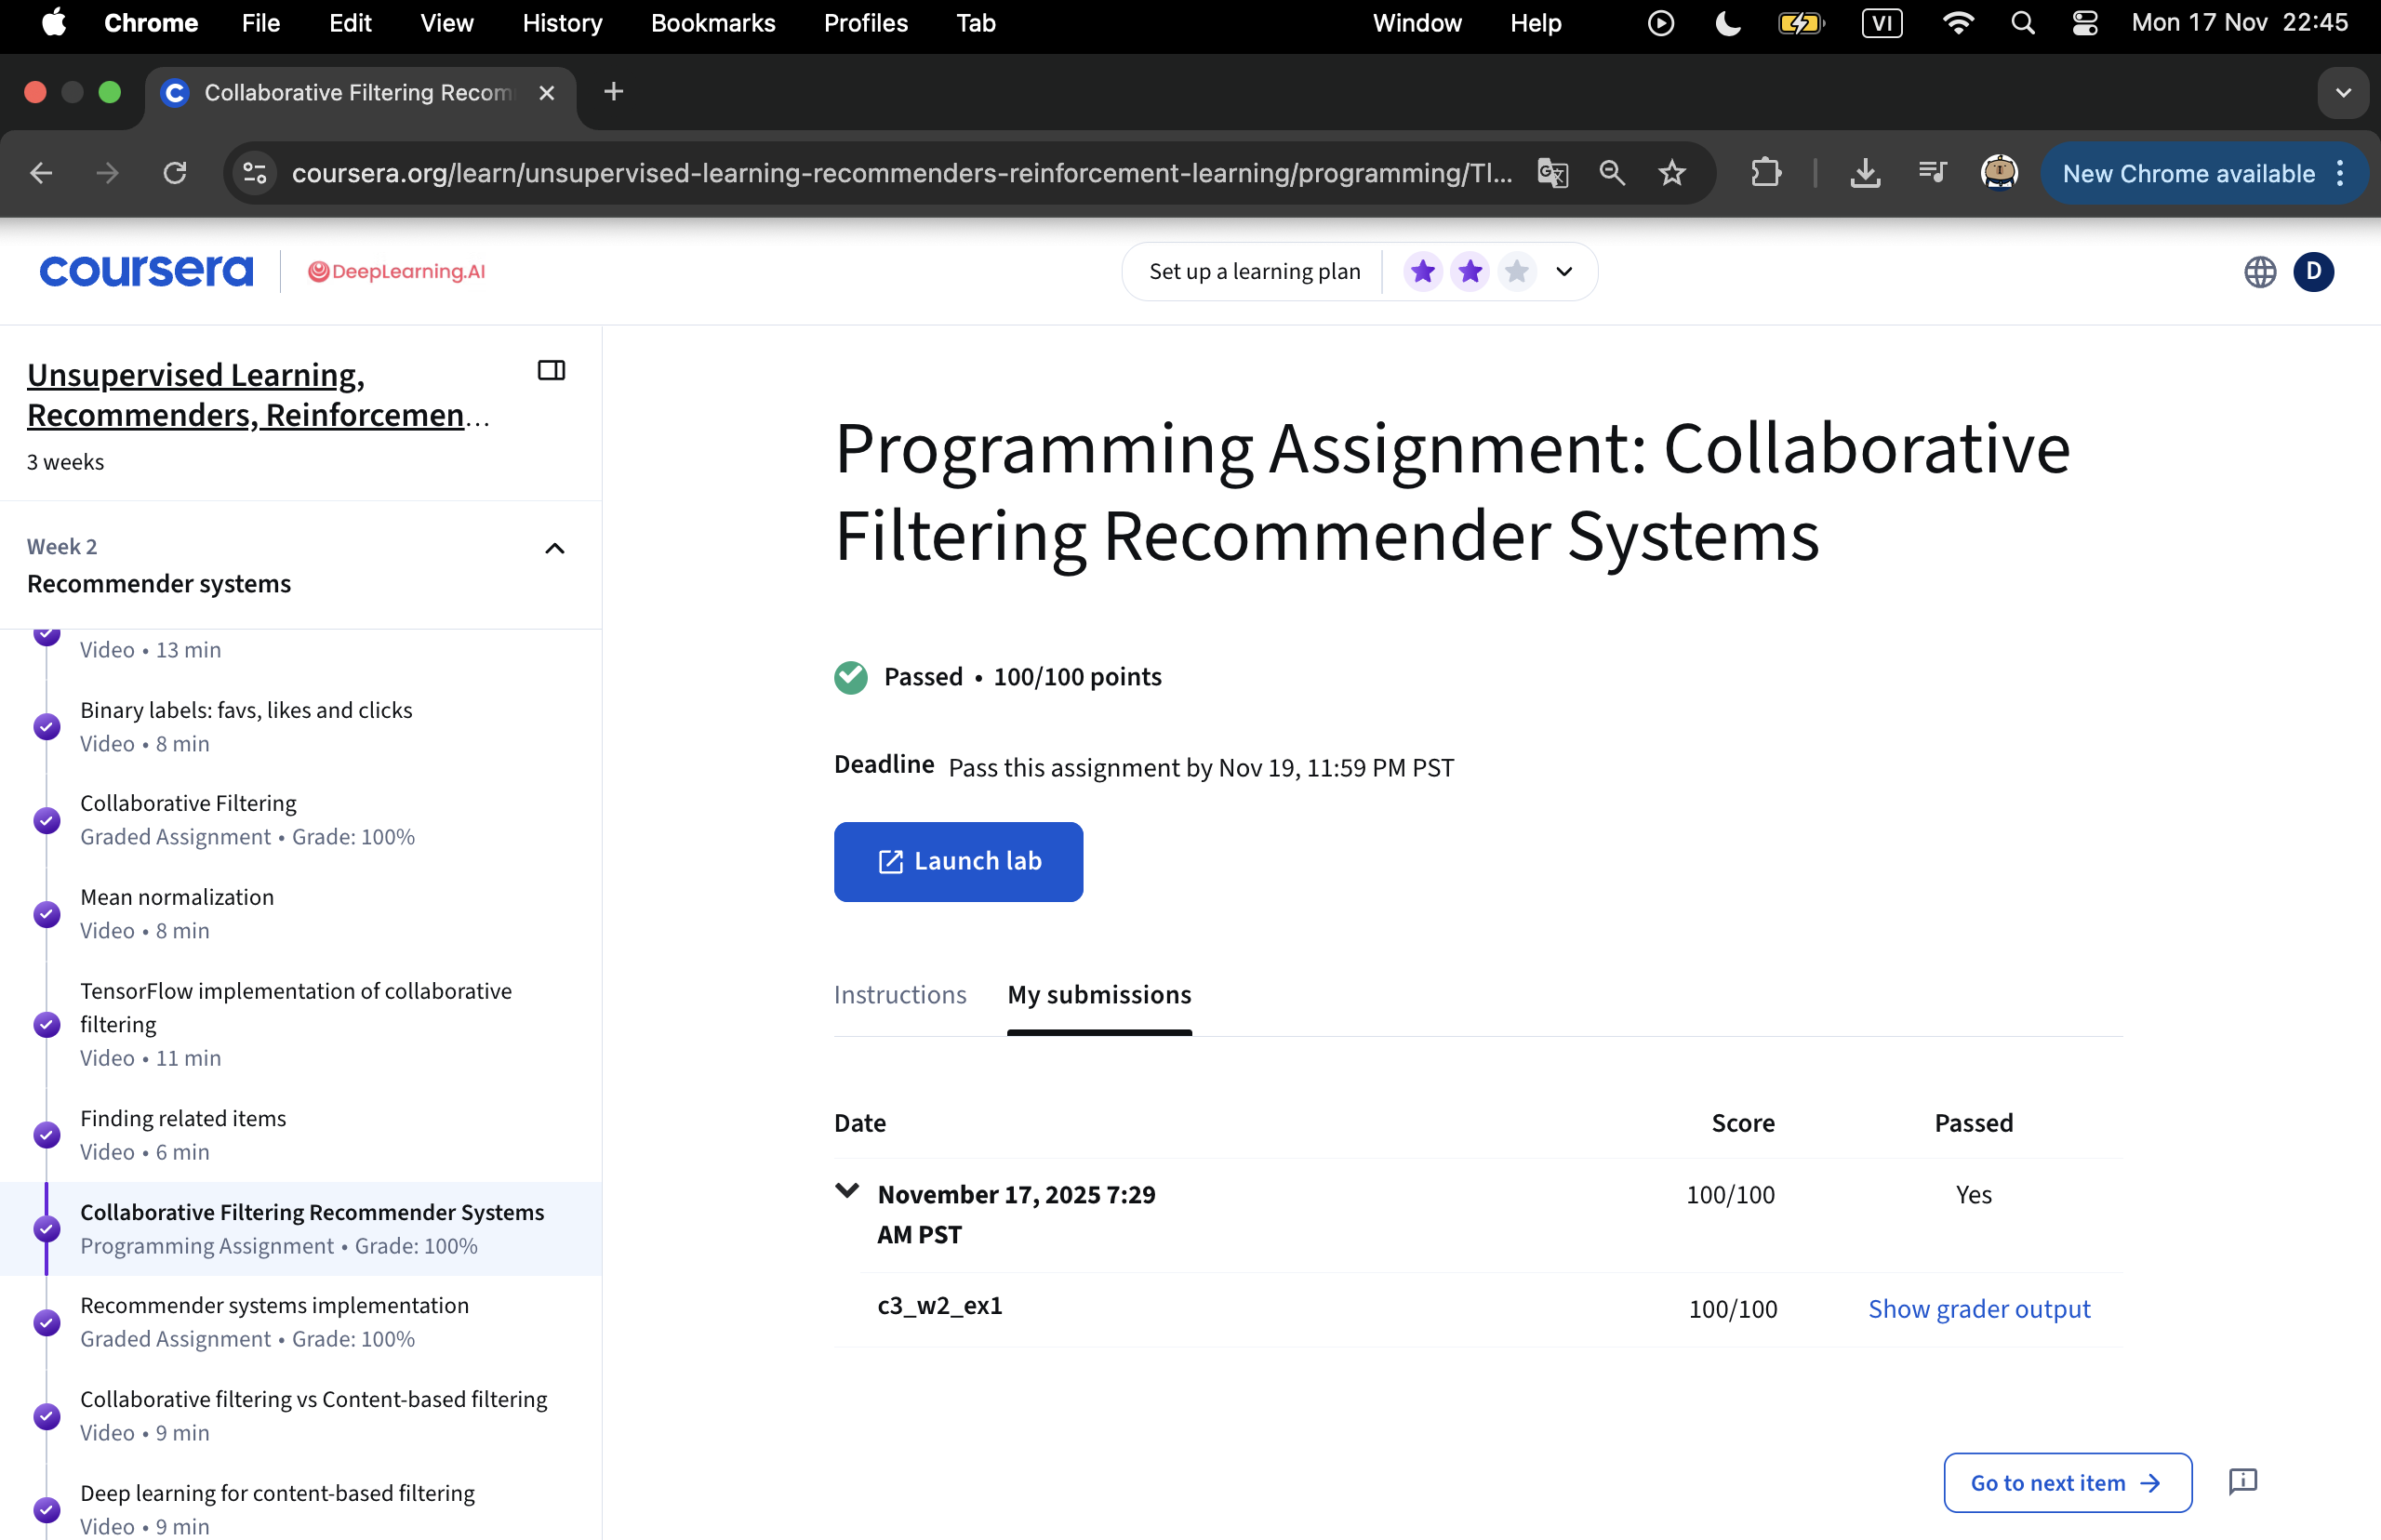
\includegraphics[scale=0.27]{Image/c3_w2_q2.png}
    \caption{Completed Programming Assignment (Collaborative Filtering Recommender Systems)}
\end{figure}

\begin{figure}[H]
    \centering
    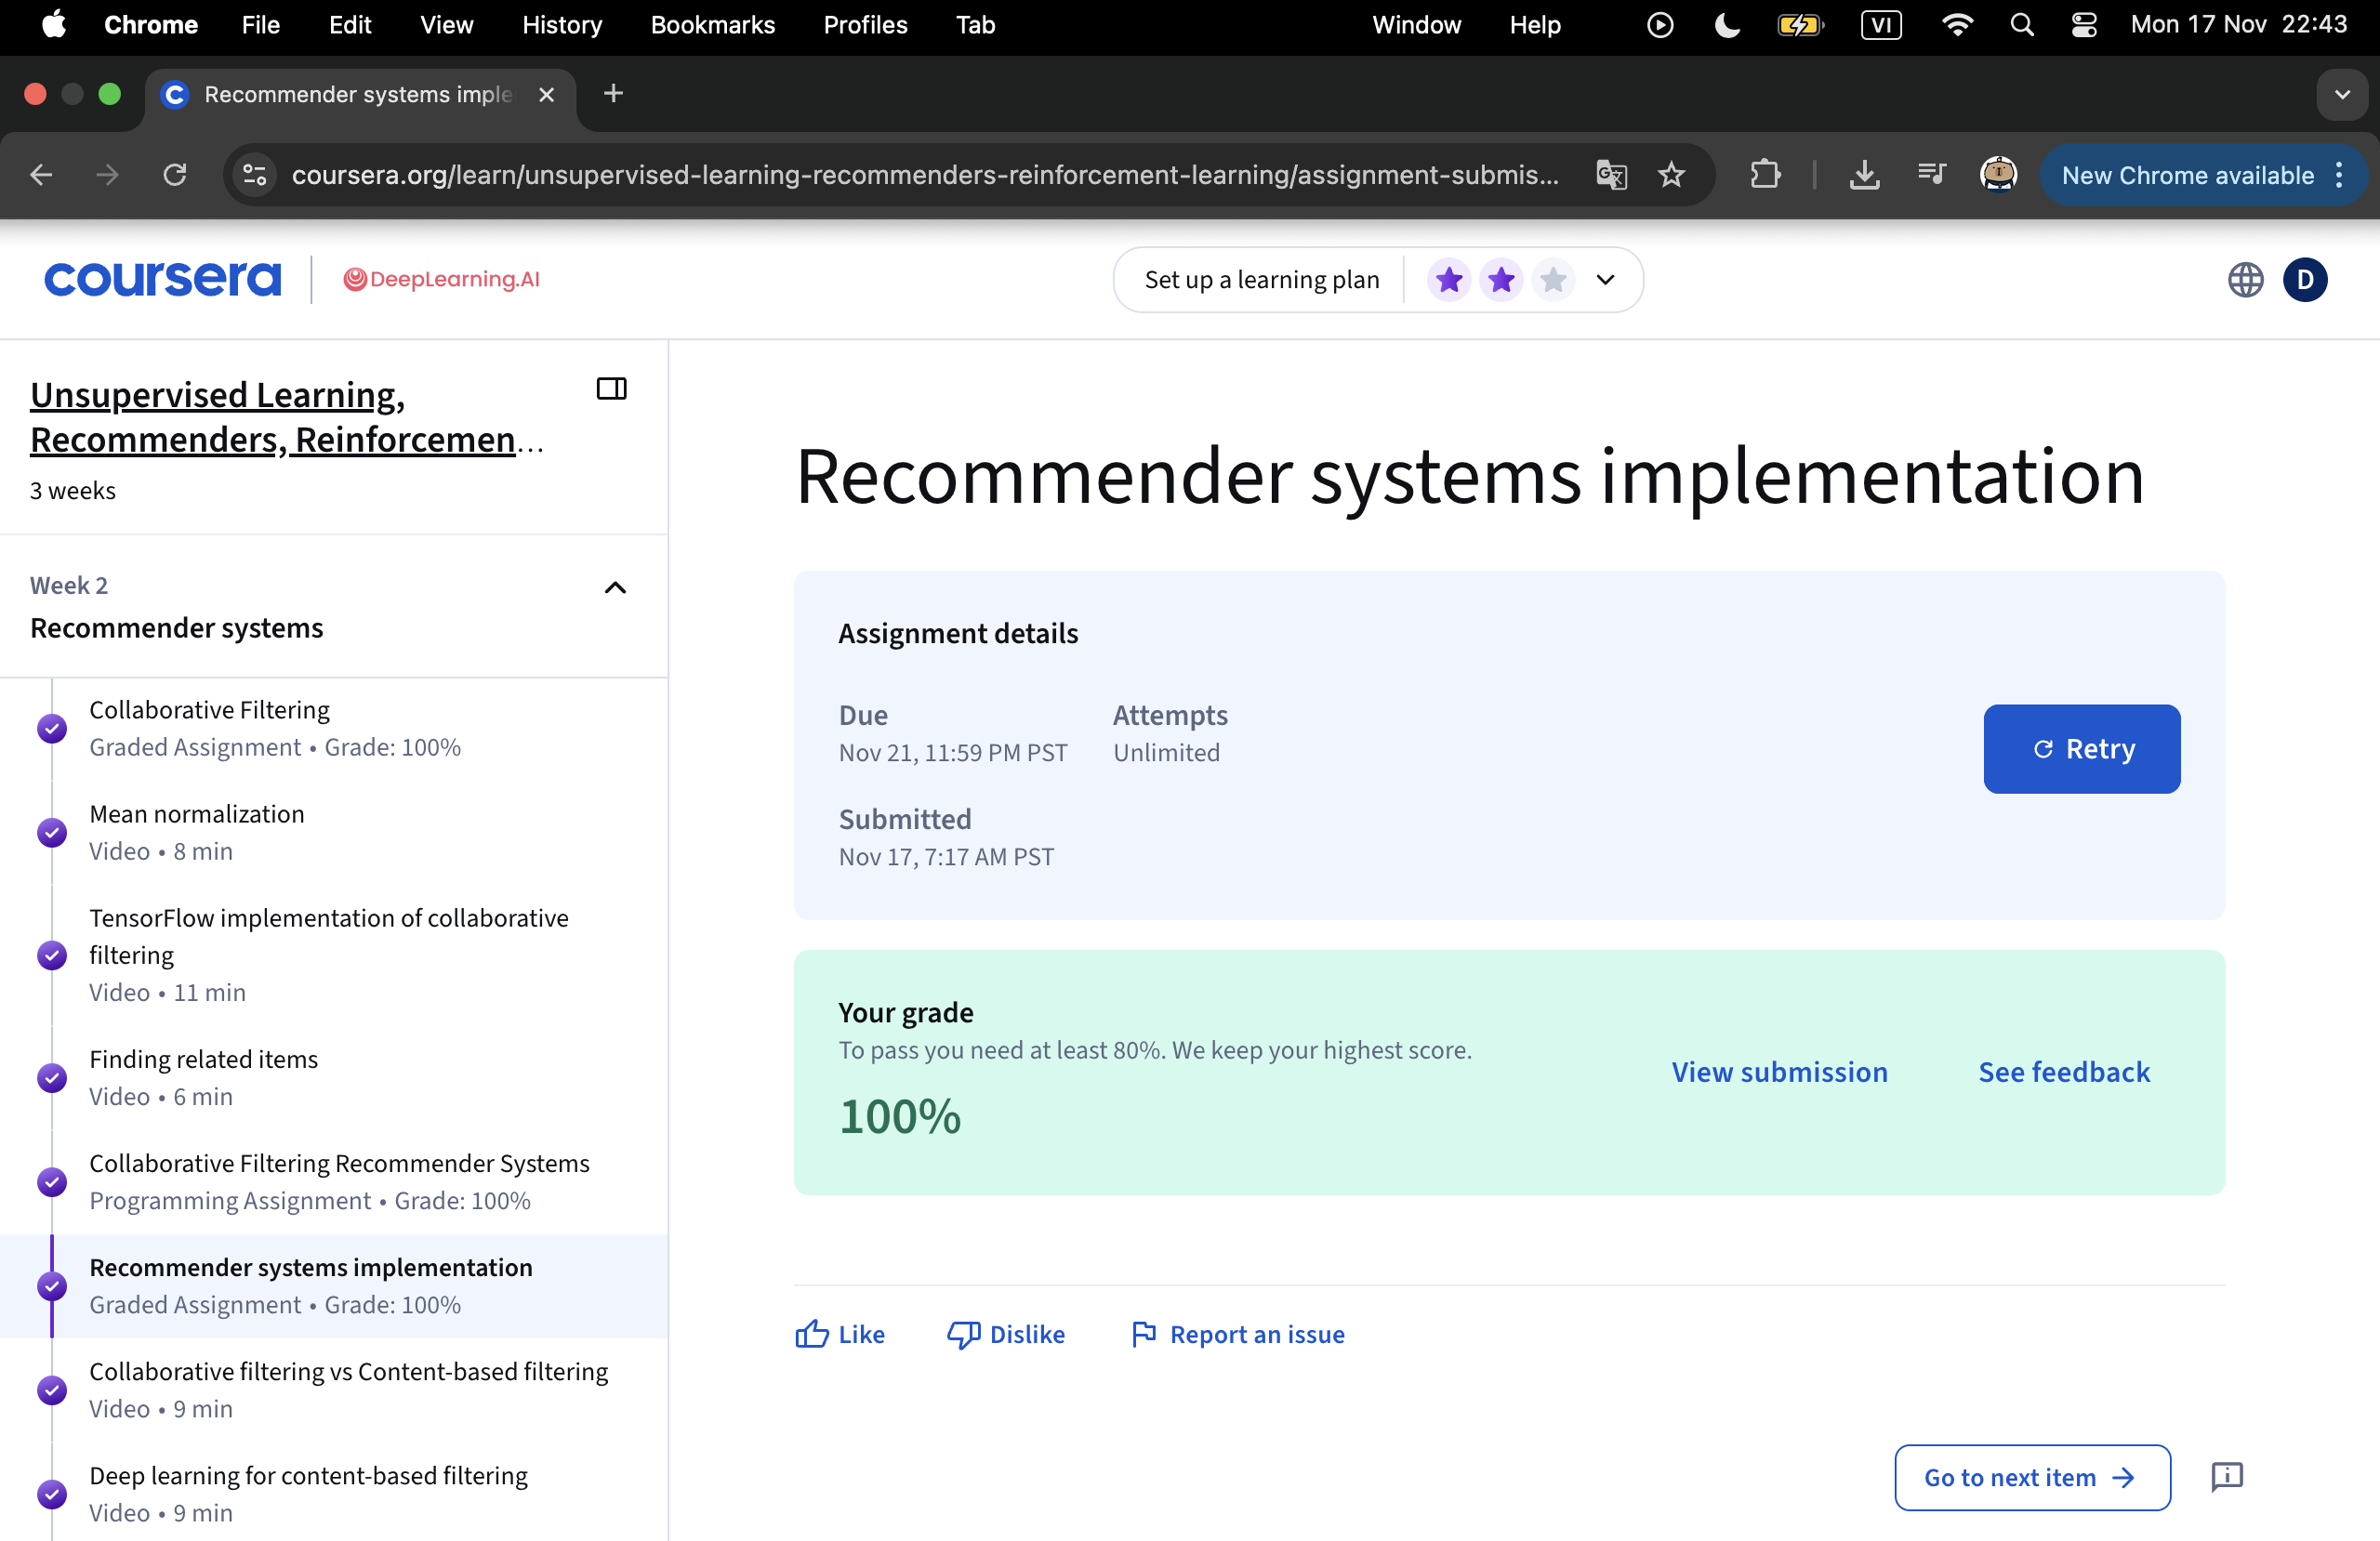
\includegraphics[scale=0.27]{Image/c3_w2_q3.png}
    \caption{Completed Graded Assignment 3 (Recommender systems implementation)}
\end{figure}

\begin{figure}[H]
    \centering
    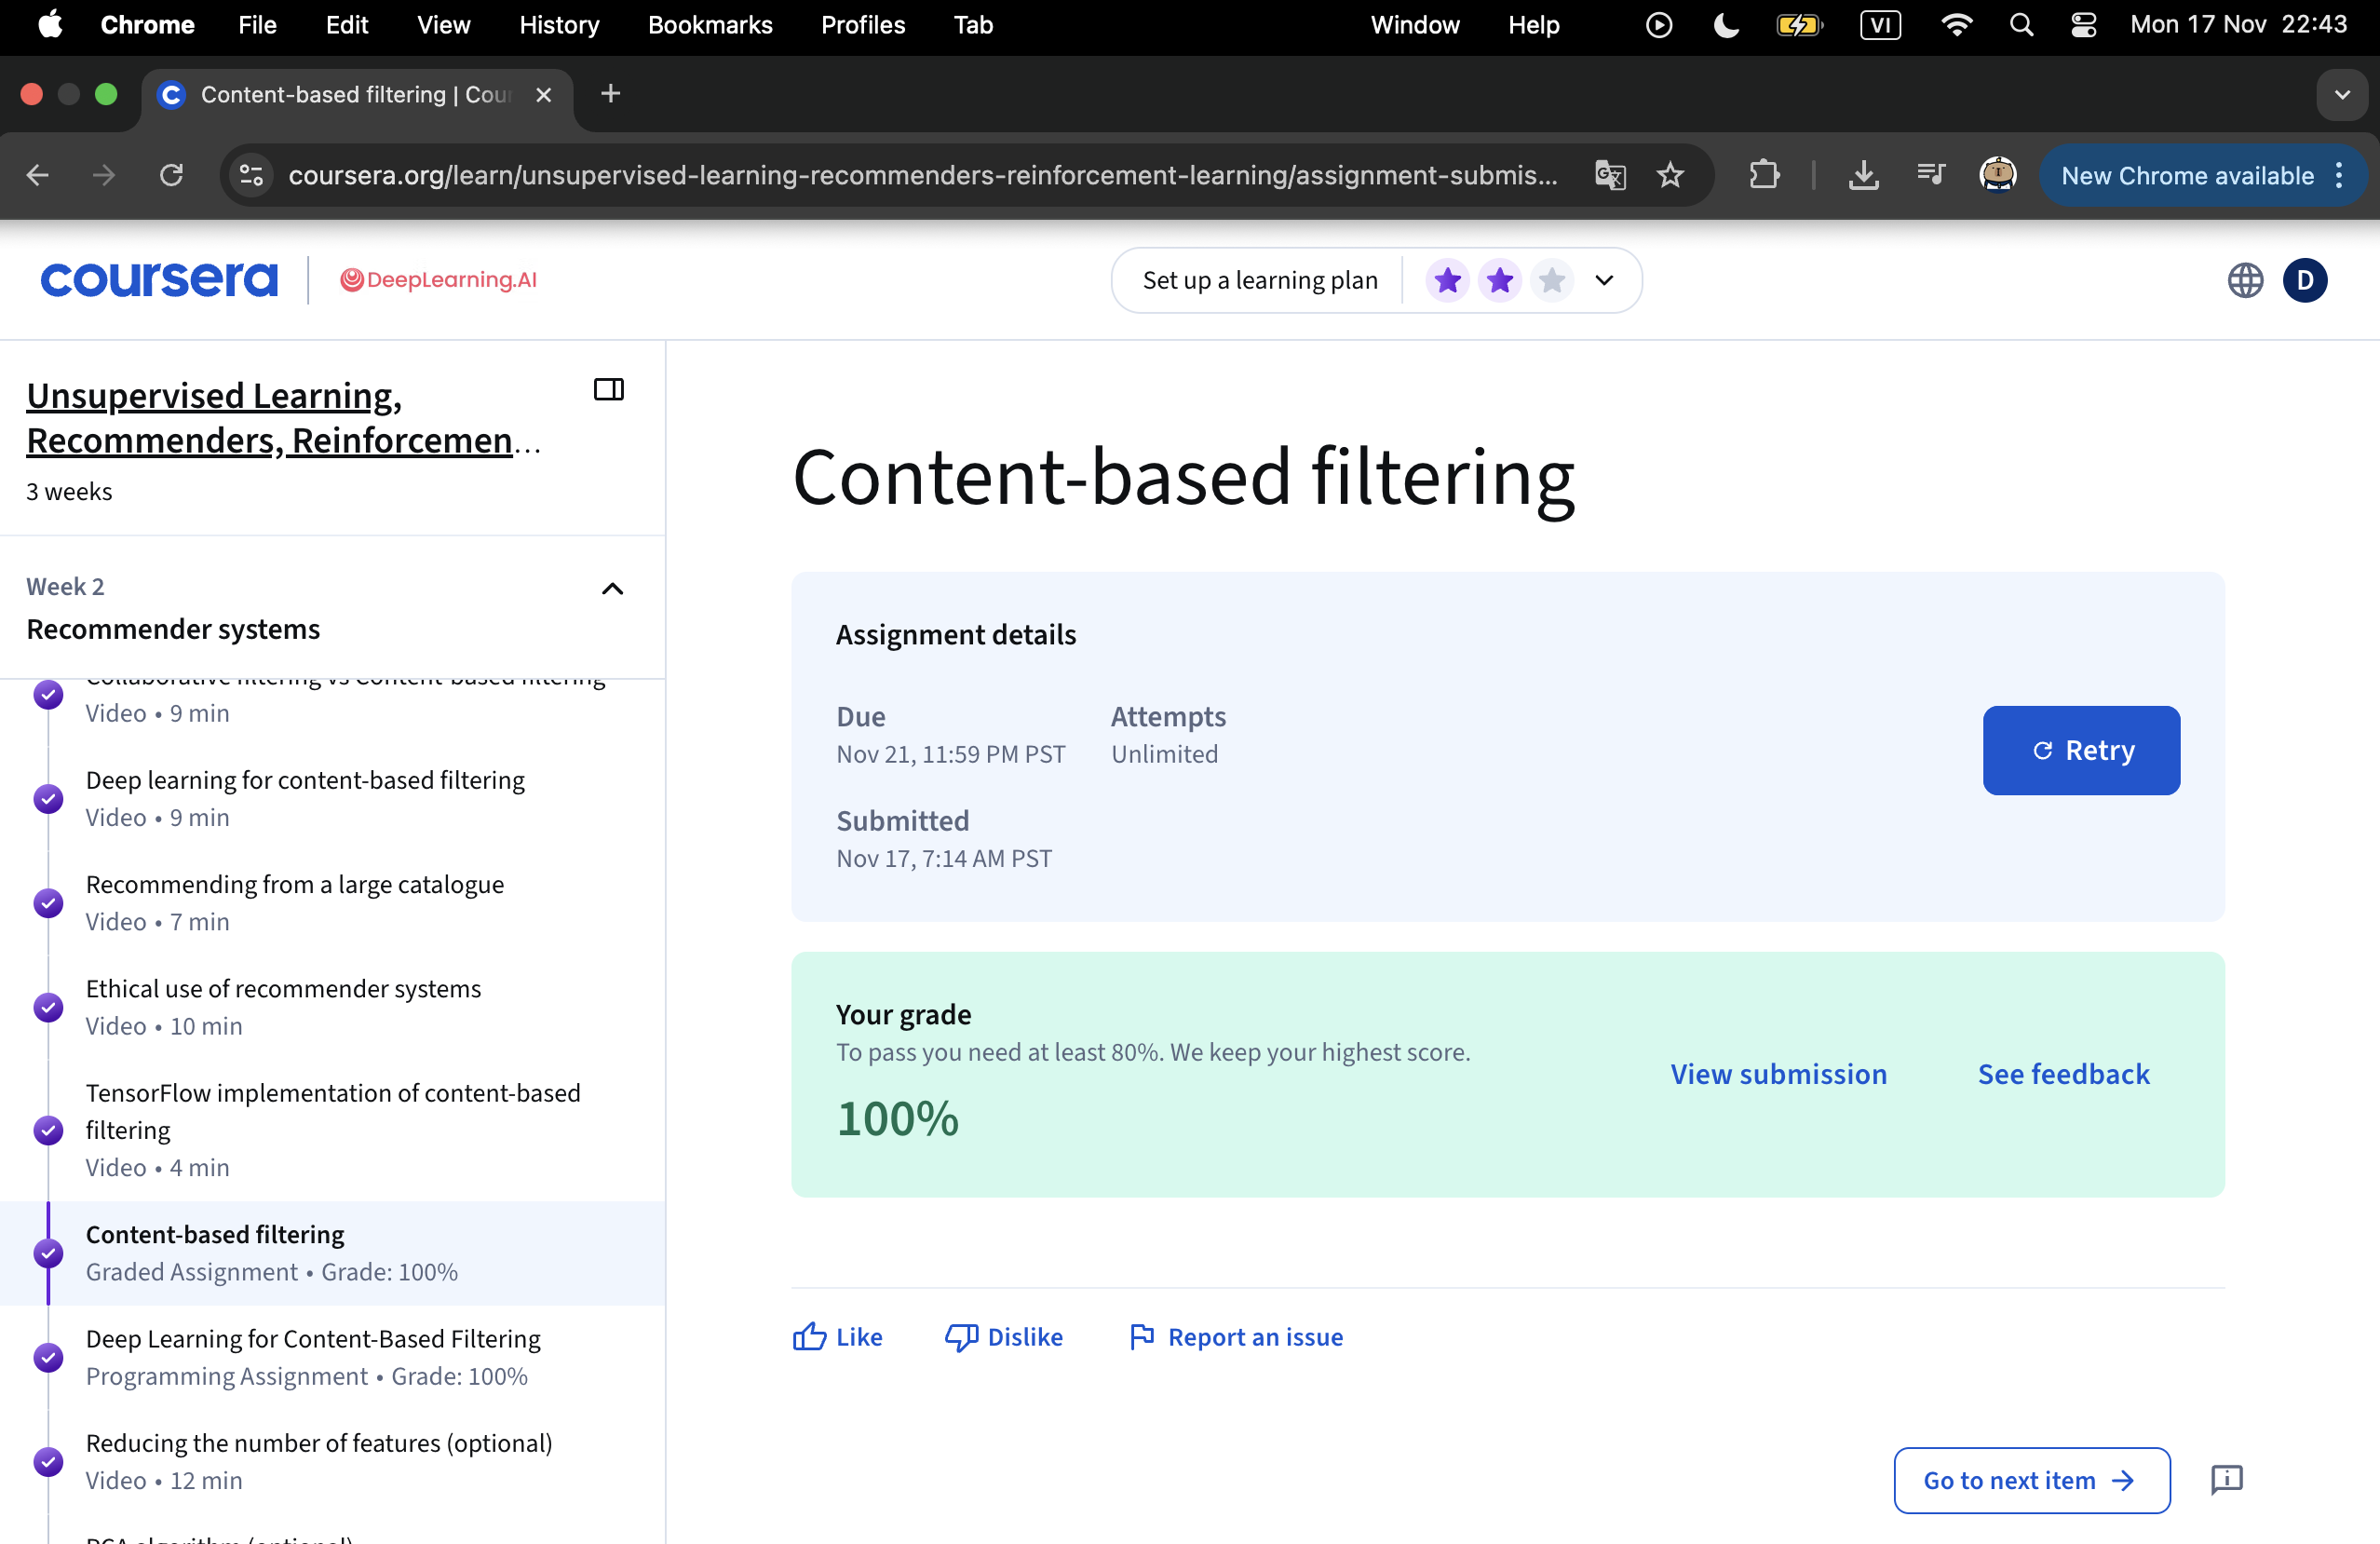
\includegraphics[scale=0.27]{Image/c3_w2_q4.png}
    \caption{Completed Graded Assignment 3 (Content-based filtering)}
\end{figure}

\begin{figure}[H]
    \centering
    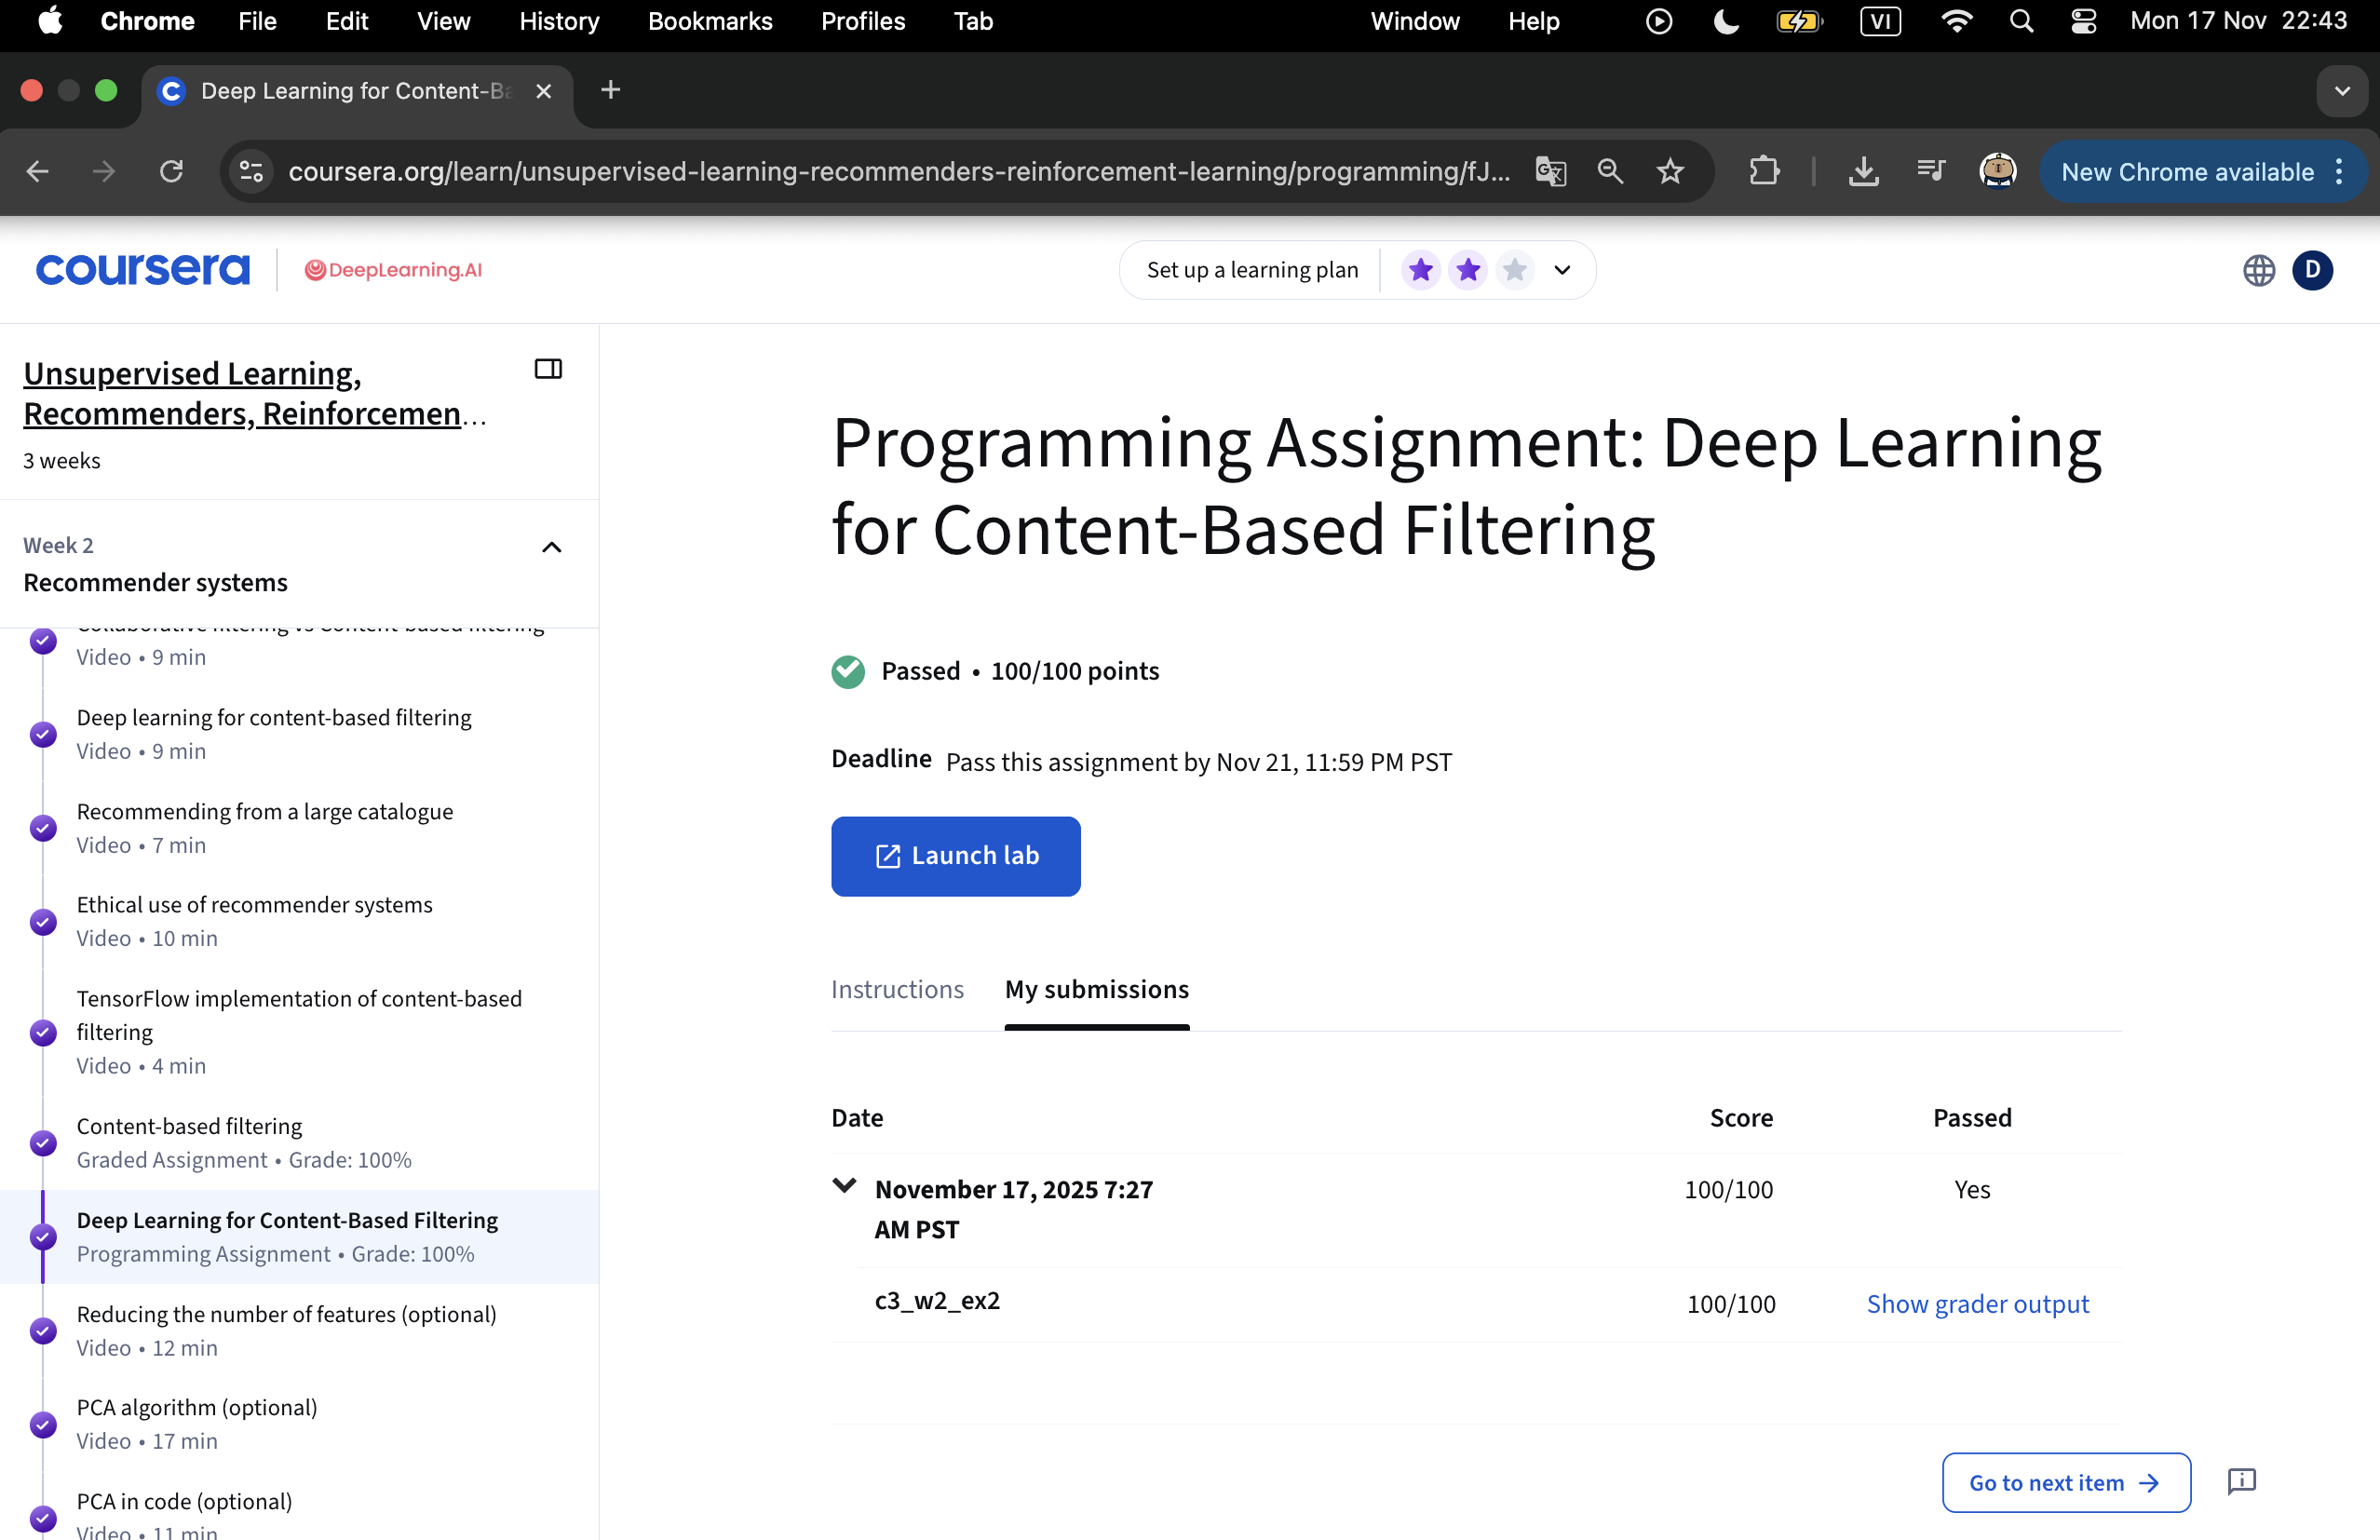
\includegraphics[scale=0.27]{Image/c3_w2_q5.png}
    \caption{Completed Programming Assignment (Deep Learning for Content-Based Filtering)}
\end{figure}


%----------------------------------------
\subsection{Week 3: Reinforcement Learning (RL)}
%----------------------------------------

\subsubsection{Key Insights and Learnings}

This module introduced a paradigm shift where an agent learns a policy to maximize rewards over time, rather than minimizing instantaneous error.

\begin{itemize}
    \item \textbf{The RL Framework (MDP):} Defined the problem as a Markov Decision Process, consisting of States ($S$), Actions ($A$), Rewards ($R$), and a Discount factor ($\gamma$). The goal is to maximize the expected \textit{Return}.
    
    \item \textbf{The Bellman Equation:} Understood the recursive relationship that defines the value of a state-action pair. This equation is the foundation for updating the Q-function to estimate long-term rewards.
    
    \item \textbf{Deep Q-Learning (DQN):} 
    \begin{itemize}
        \item Replaced traditional Q-tables with Neural Networks to approximate the Q-function, enabling the agent to handle complex, high-dimensional state spaces (e.g., video game pixels or robot sensors).
        \item \textbf{Exploration vs. Exploitation:} Implemented the $\epsilon$-greedy policy to balance trying new actions versus leveraging known optimal actions.
    \end{itemize}
\end{itemize}

\subsubsection{Learning Evidence}
\begin{figure}[H]
    \centering
    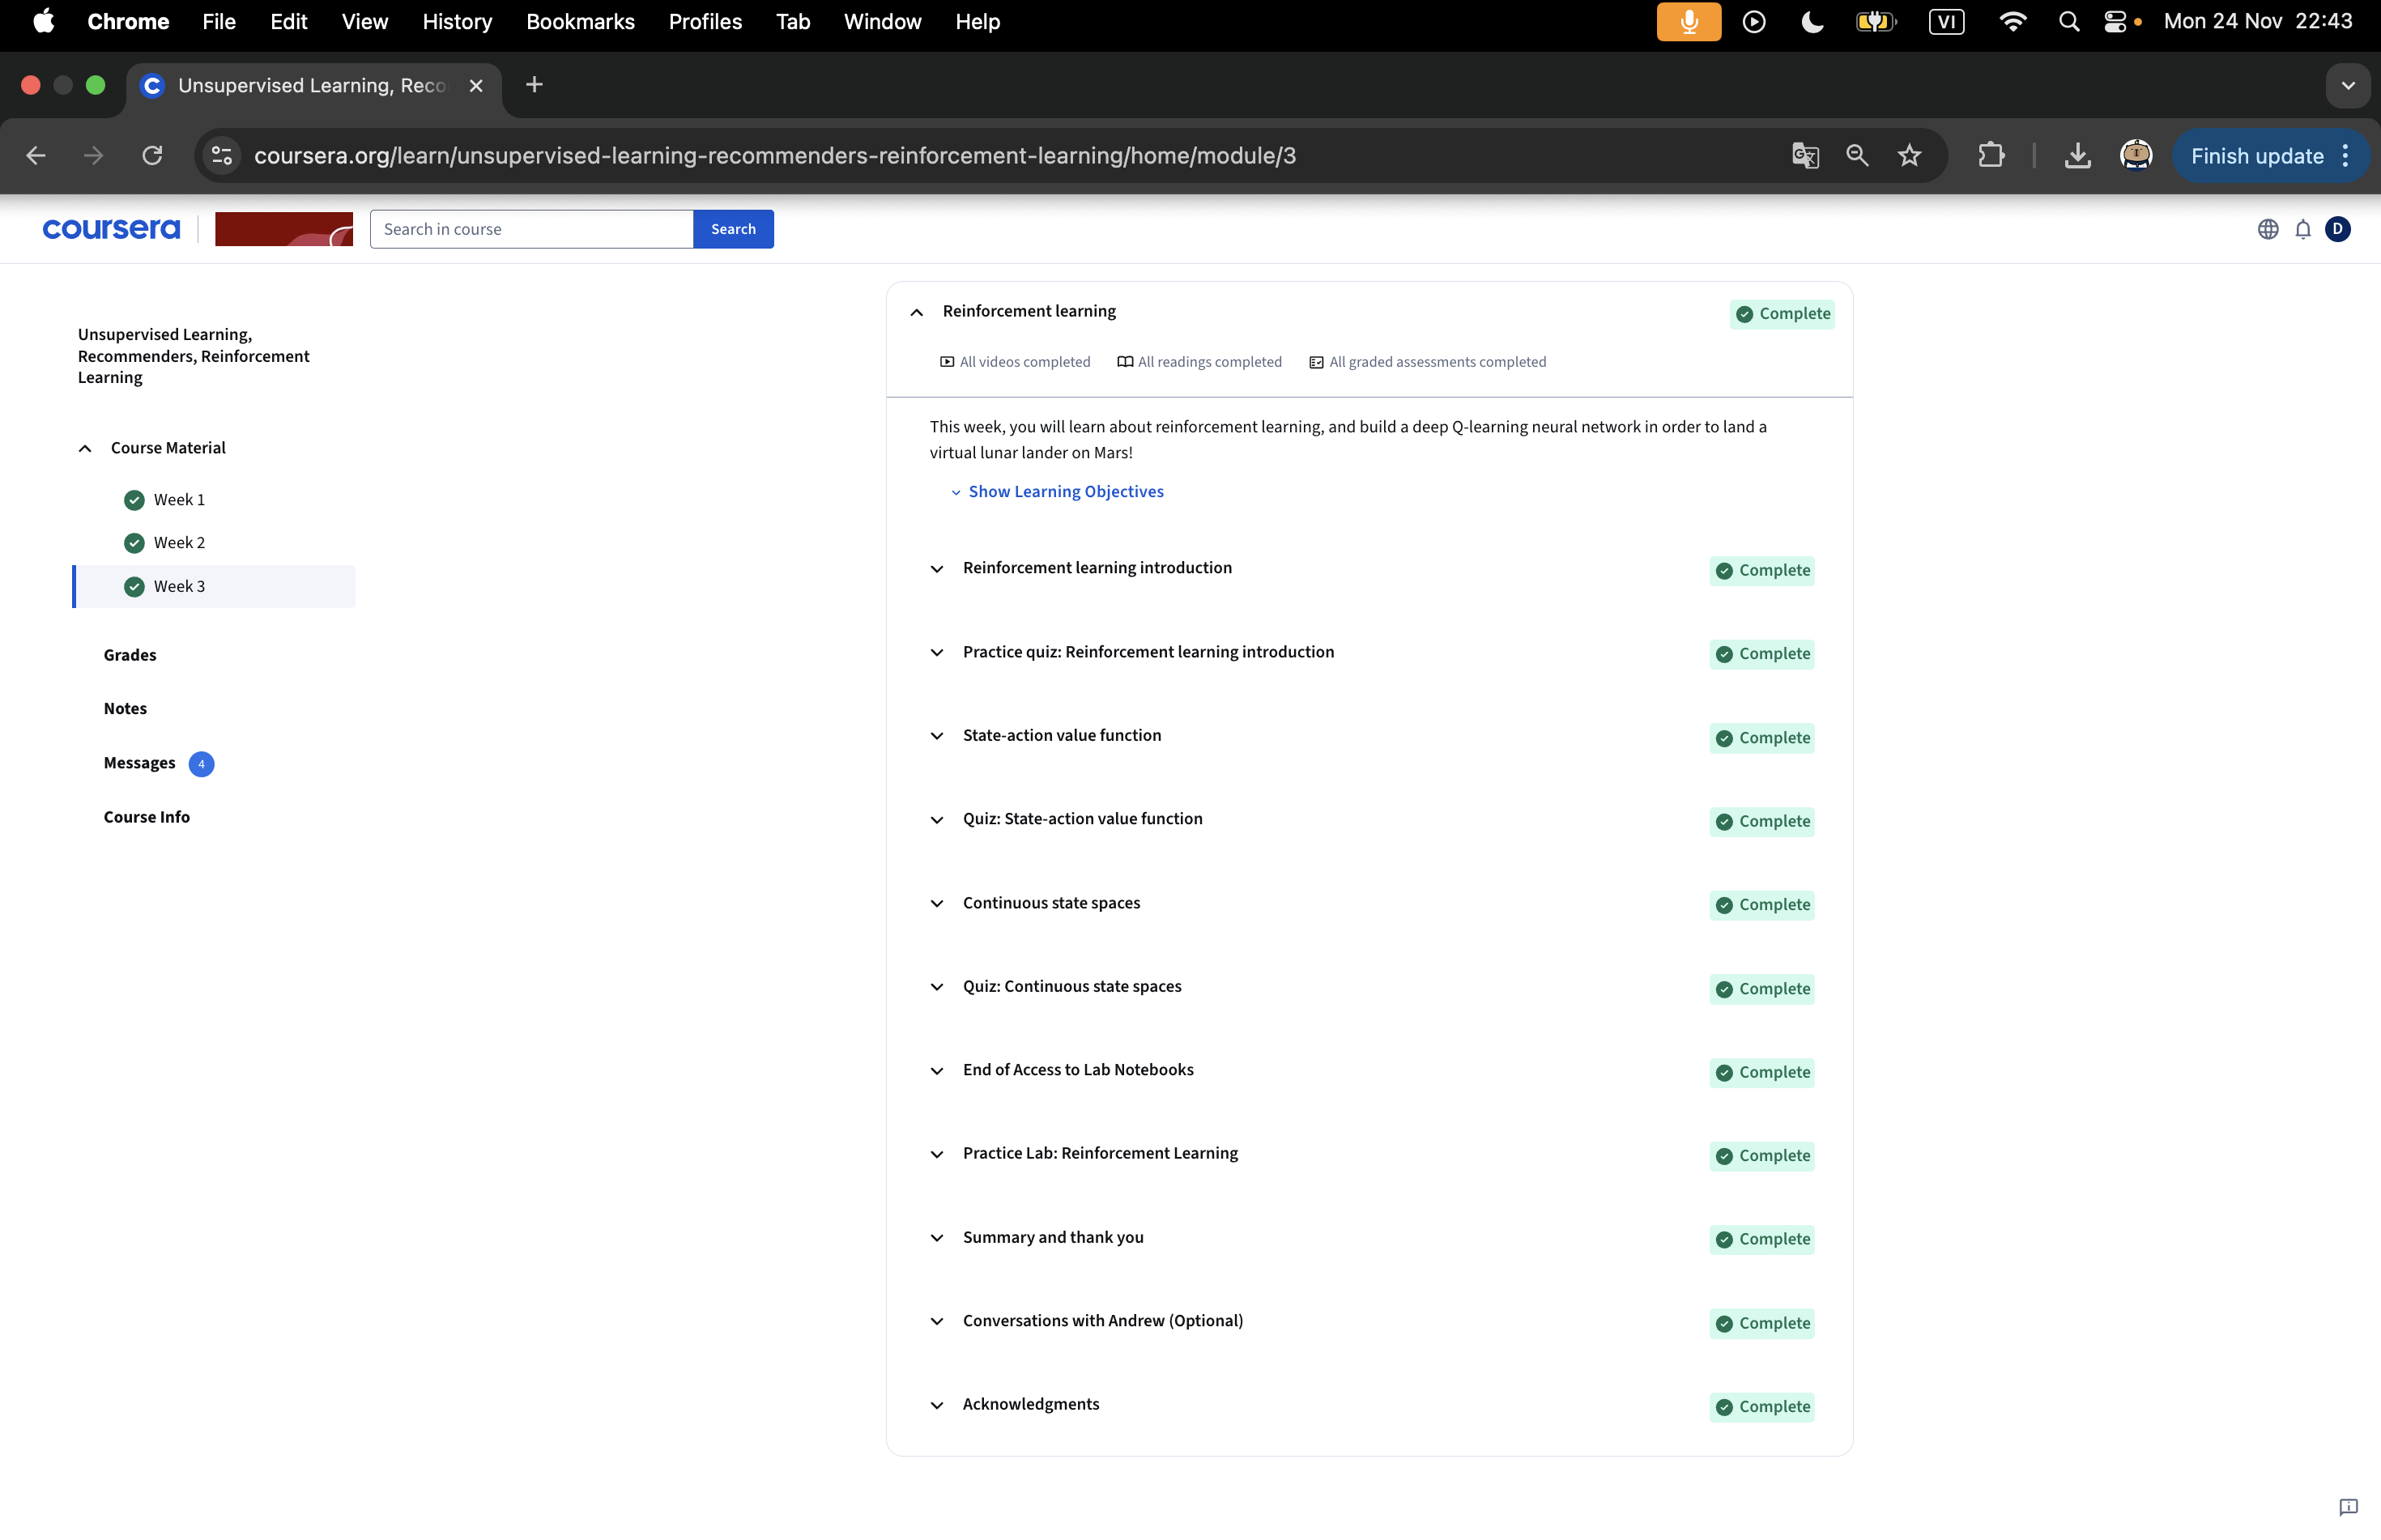
\includegraphics[scale=0.25]{Image/c3_w3.png}
    \caption{Lesson's completed date (24/11/2025)}
\end{figure}

\subsubsection{Graded Assignment Evidence}
\begin{figure}[H]
    \centering
    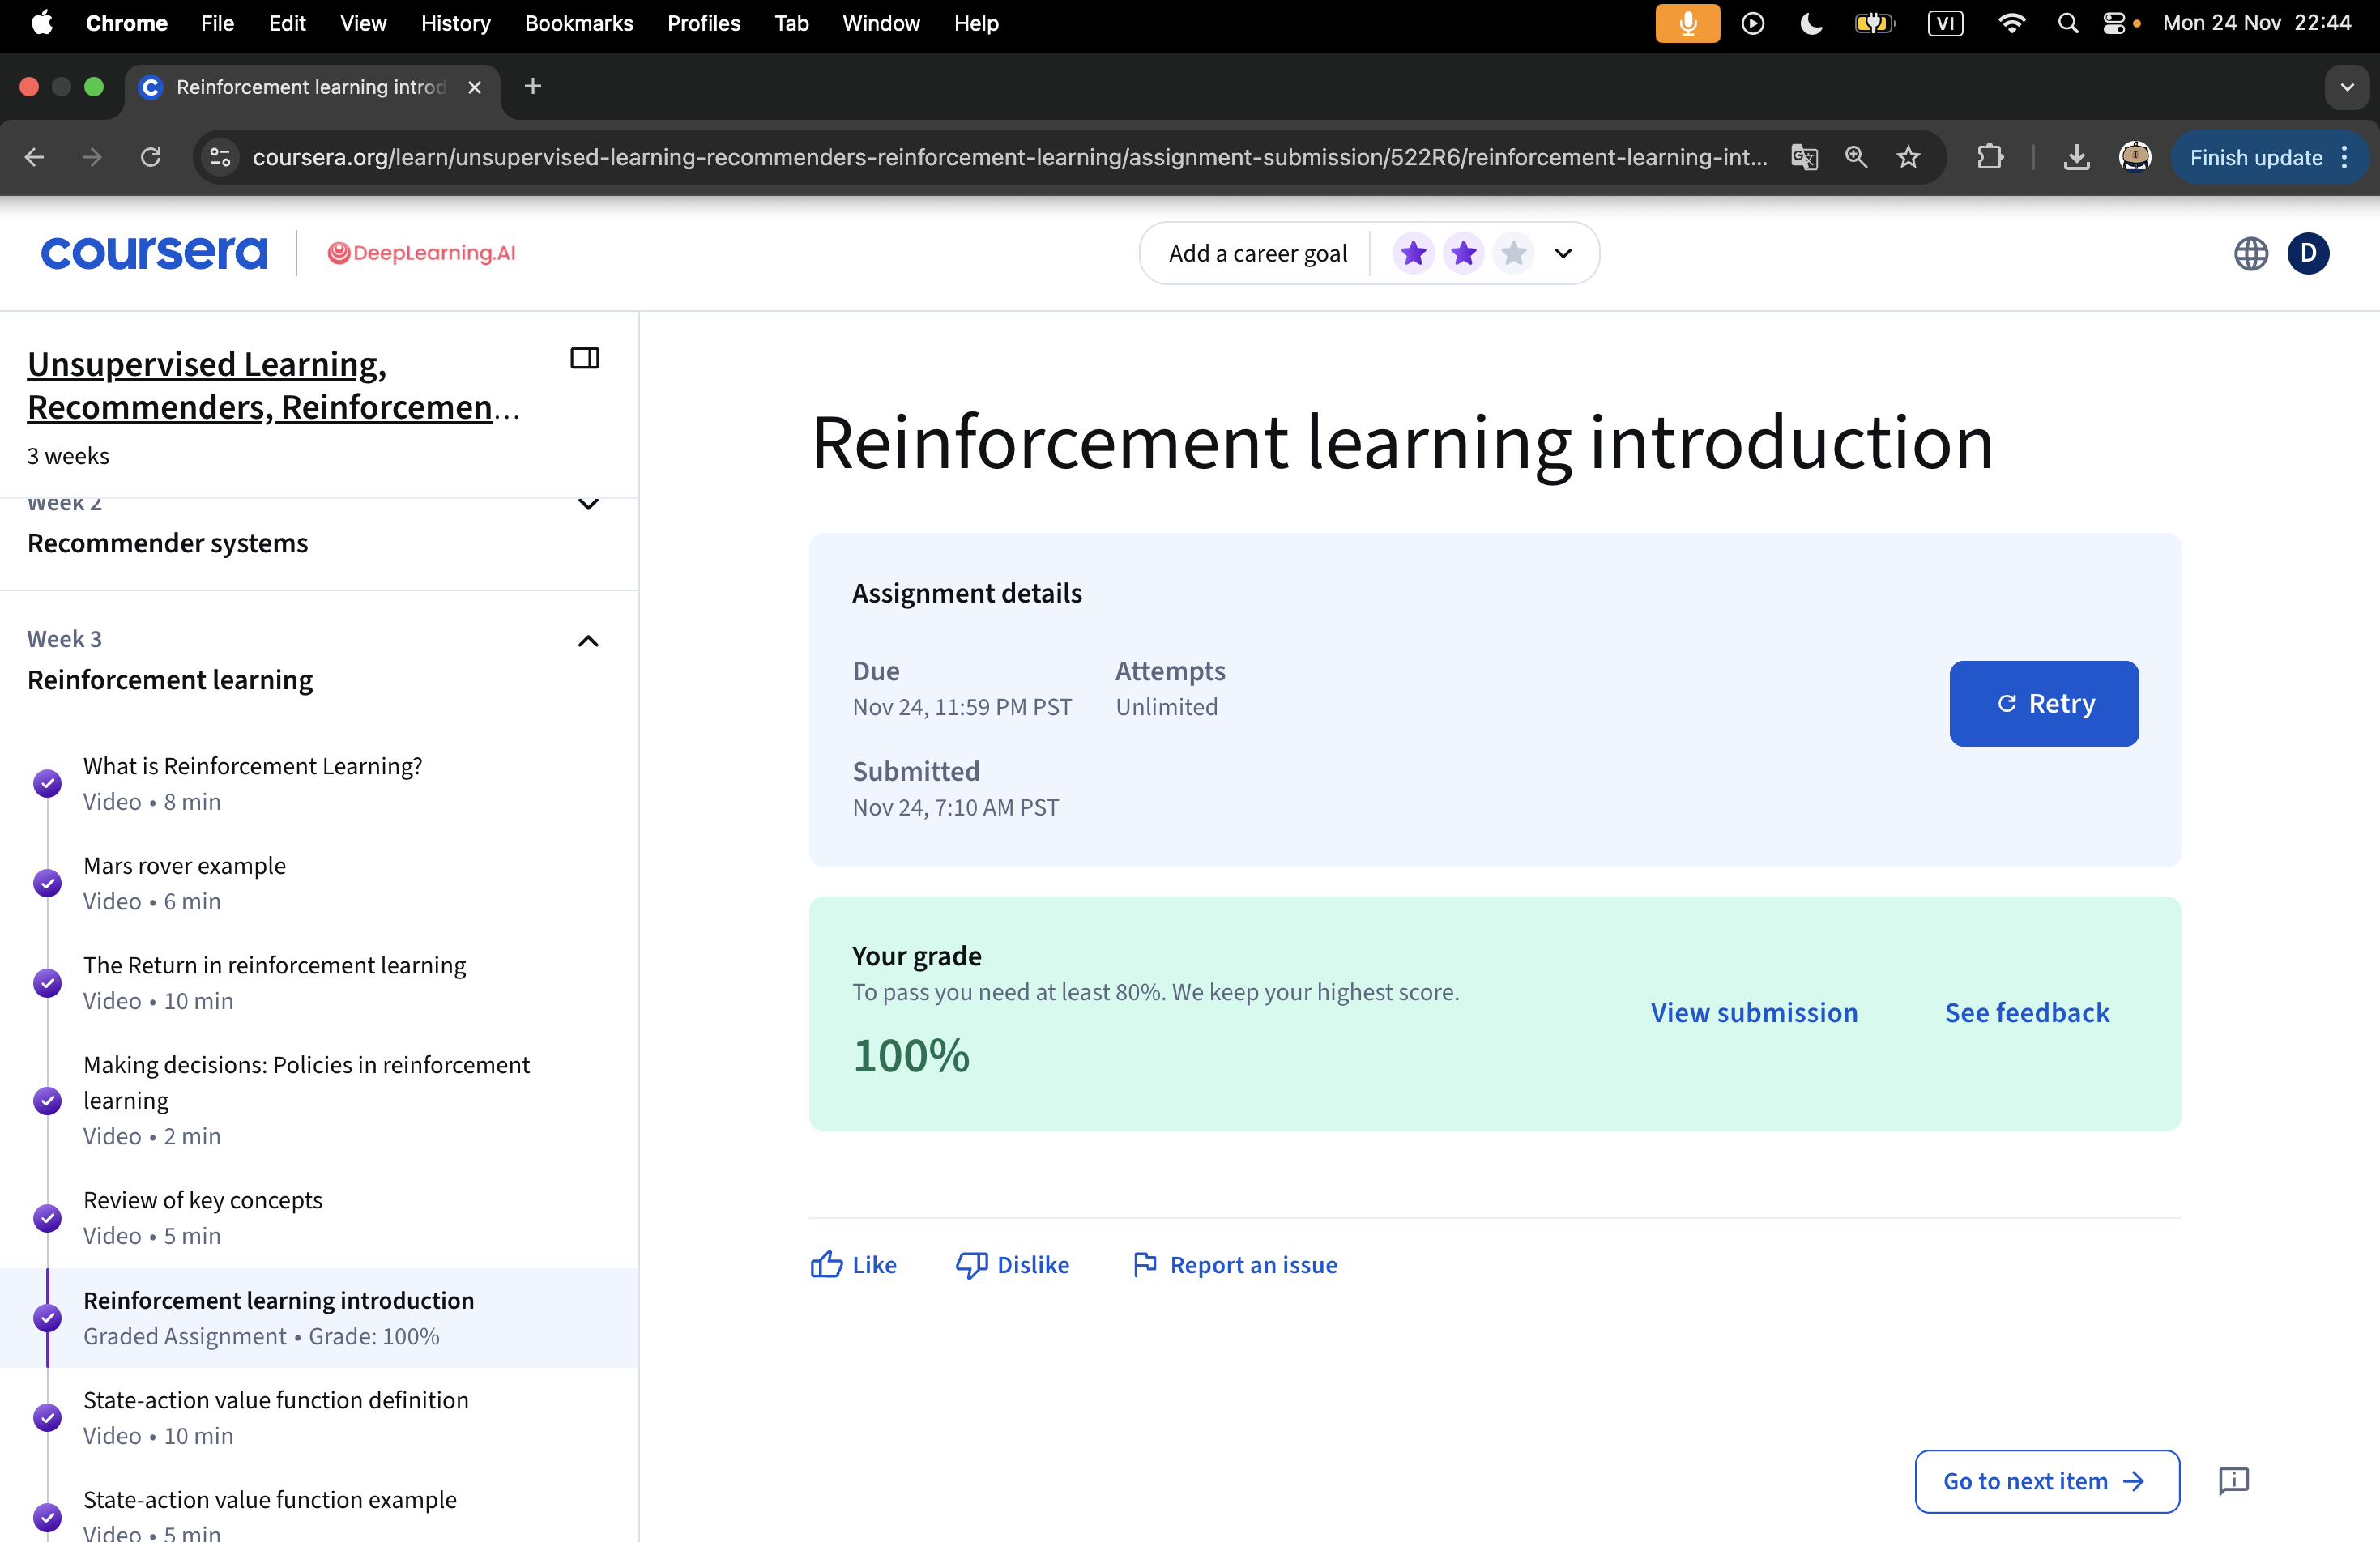
\includegraphics[scale=0.25]{Image/c3_w3_q1.png}
    \caption{Completed Graded Assignment 1 (Reinforcement learning introduction)}
\end{figure}

\begin{figure}[H]
    \centering
    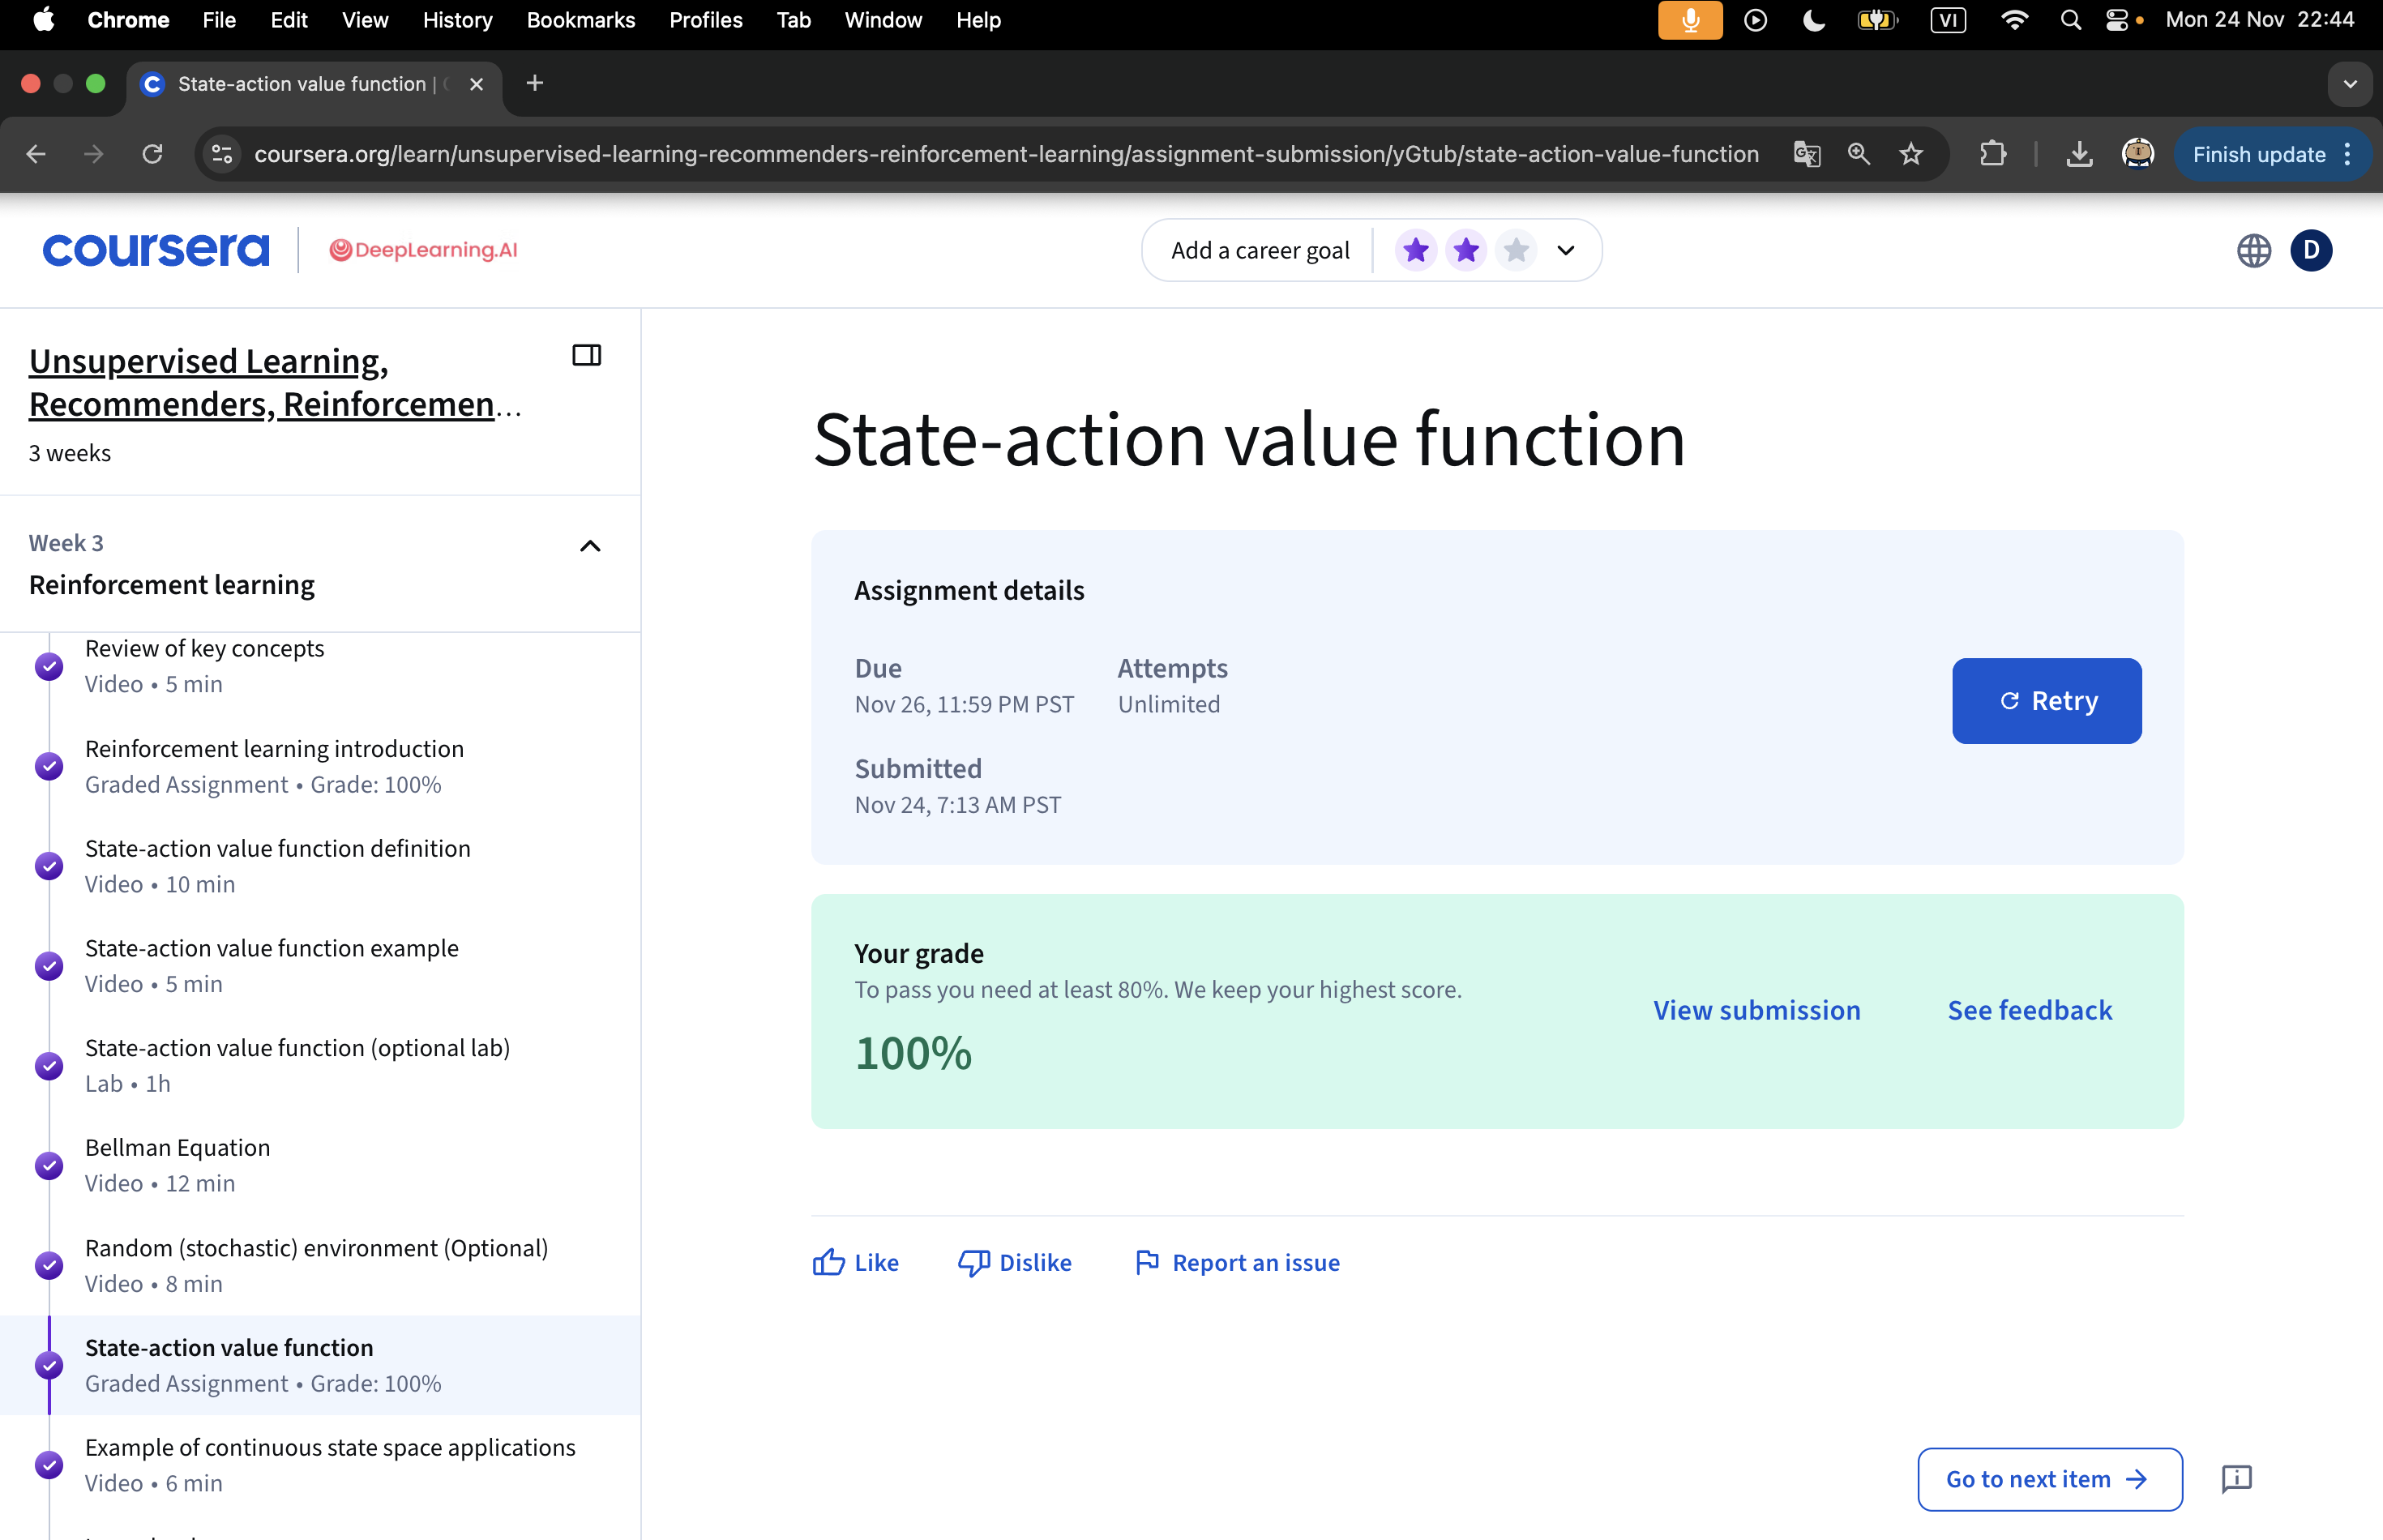
\includegraphics[scale=0.25]{Image/c3_w3_q2.png}
    \caption{Completed Graded Assignment 2 (State-action value function)}
\end{figure}

\begin{figure}[H]
    \centering
    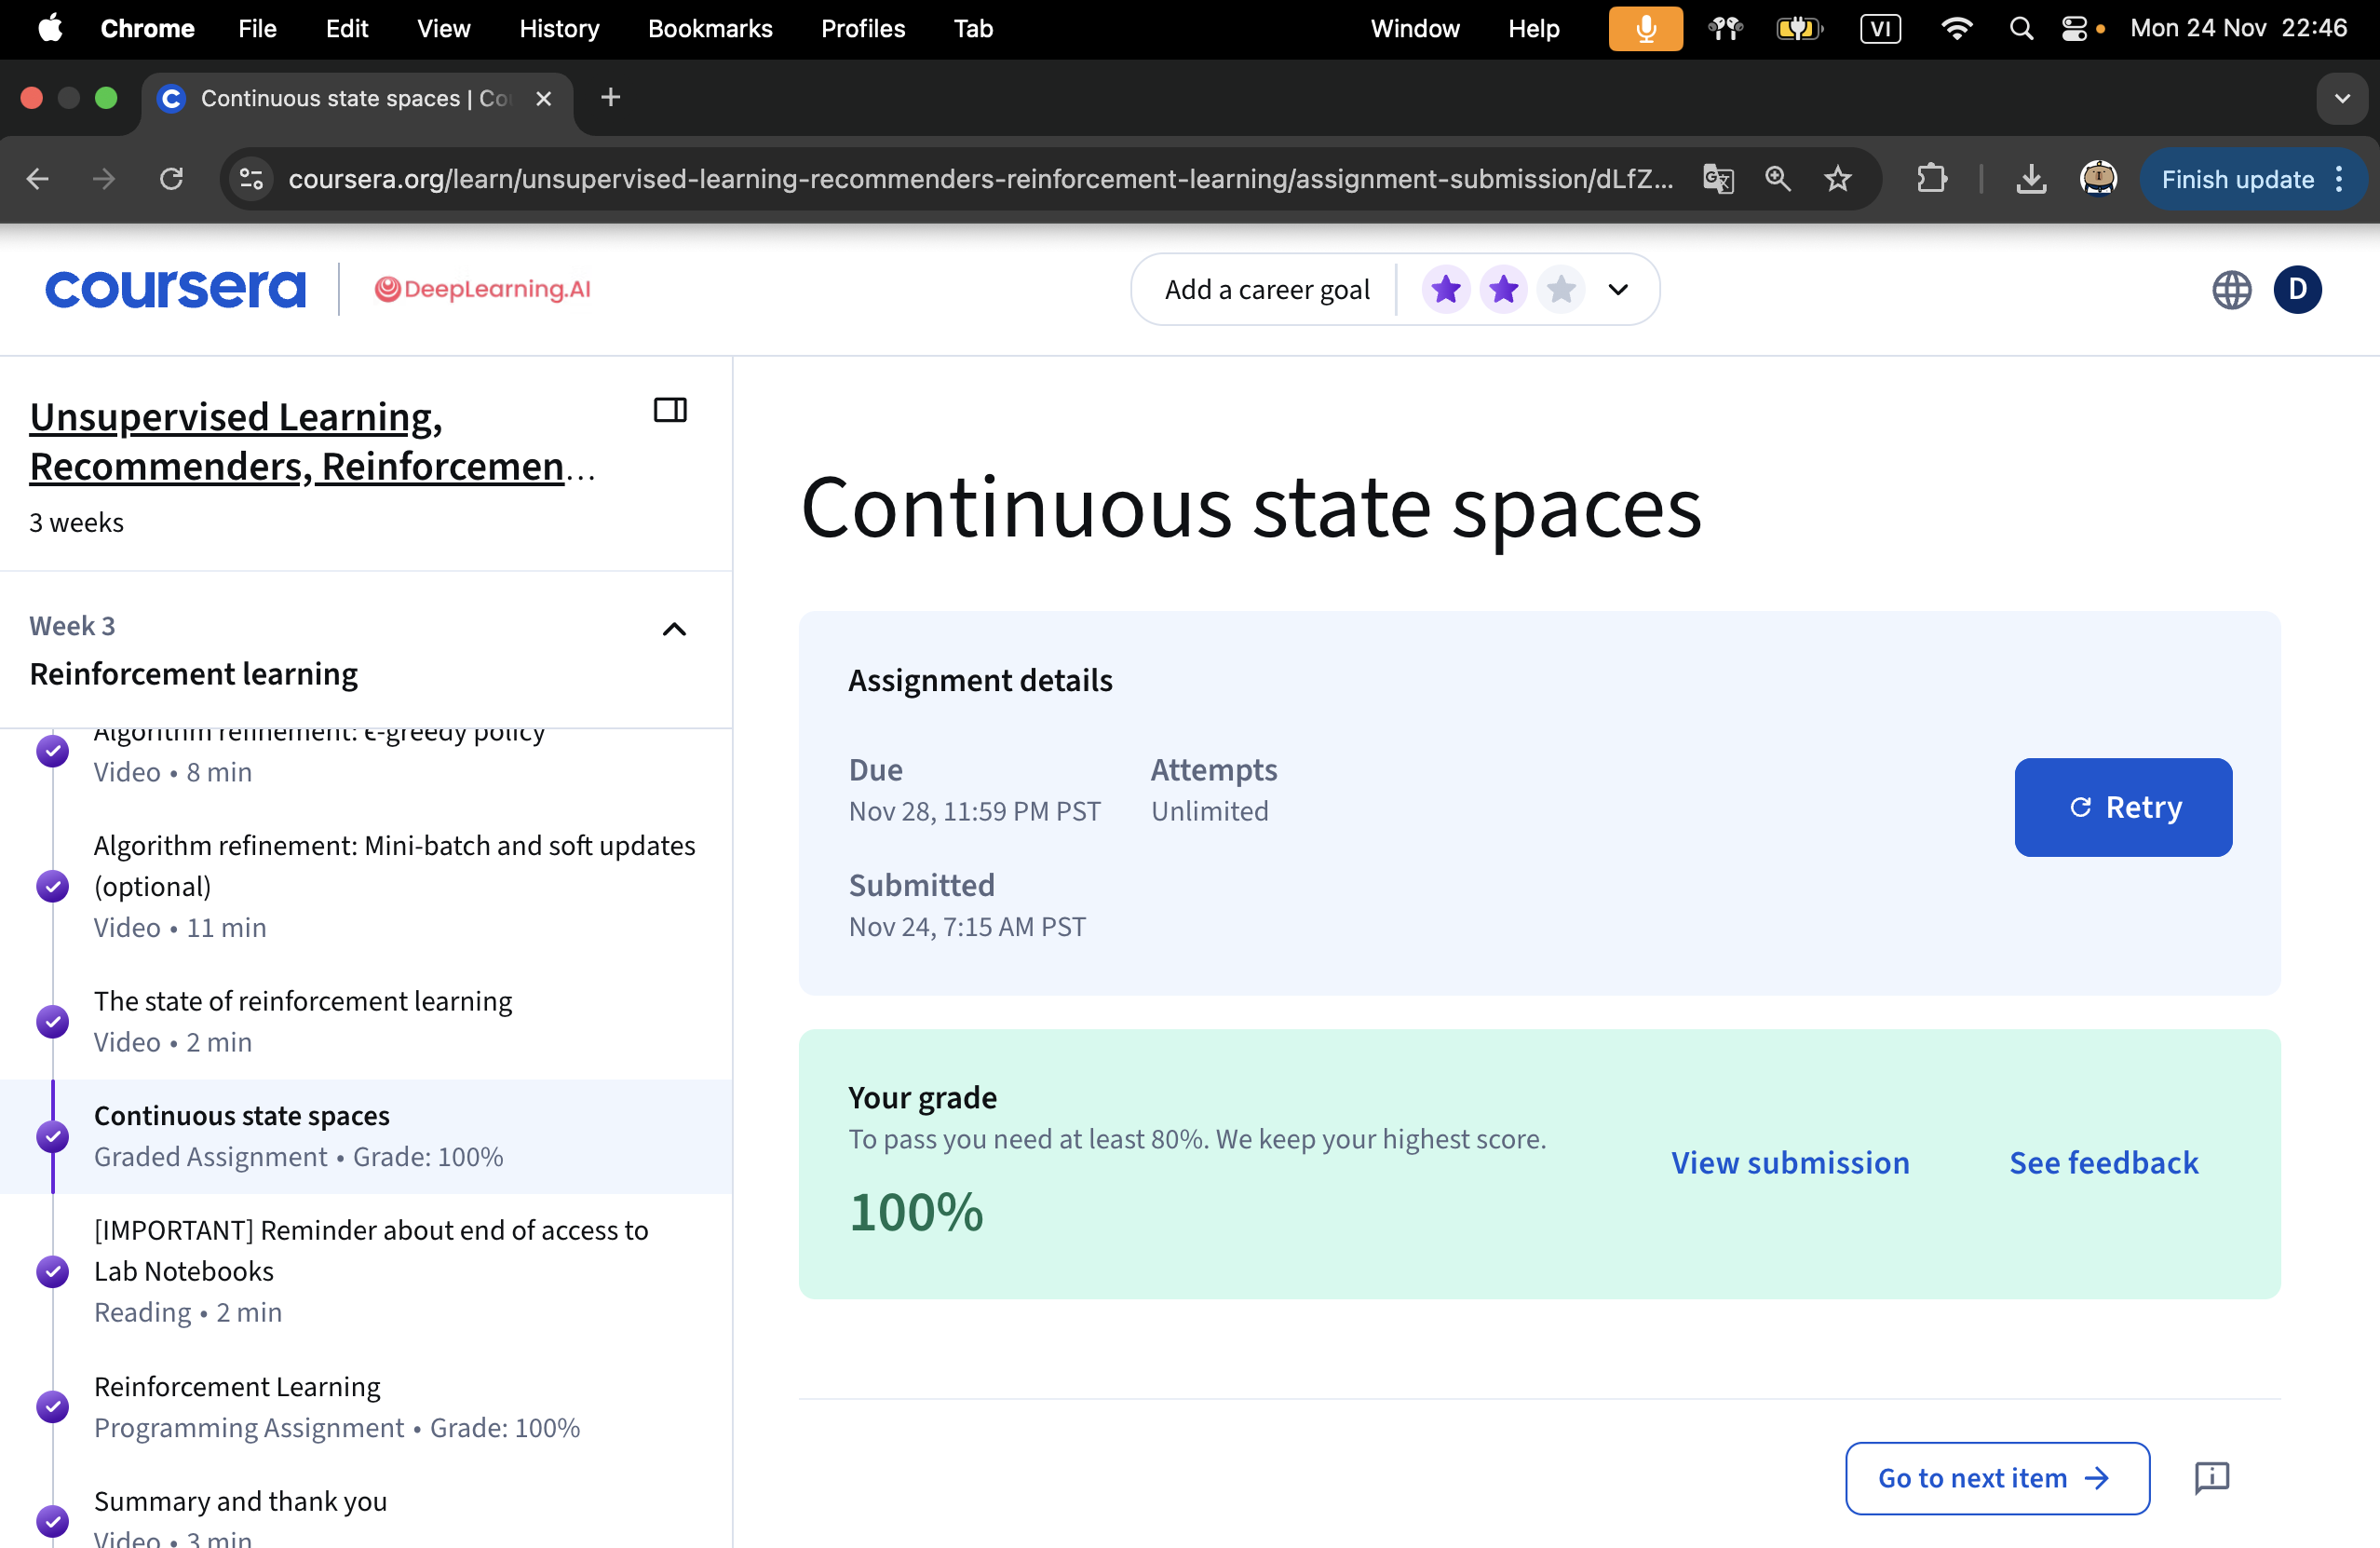
\includegraphics[scale=0.25]{Image/c3_w3_q3.png}
    \caption{Completed Graded Assignment 3 (Continuous state spaces)}
\end{figure}


\begin{figure}[H]
    \centering
    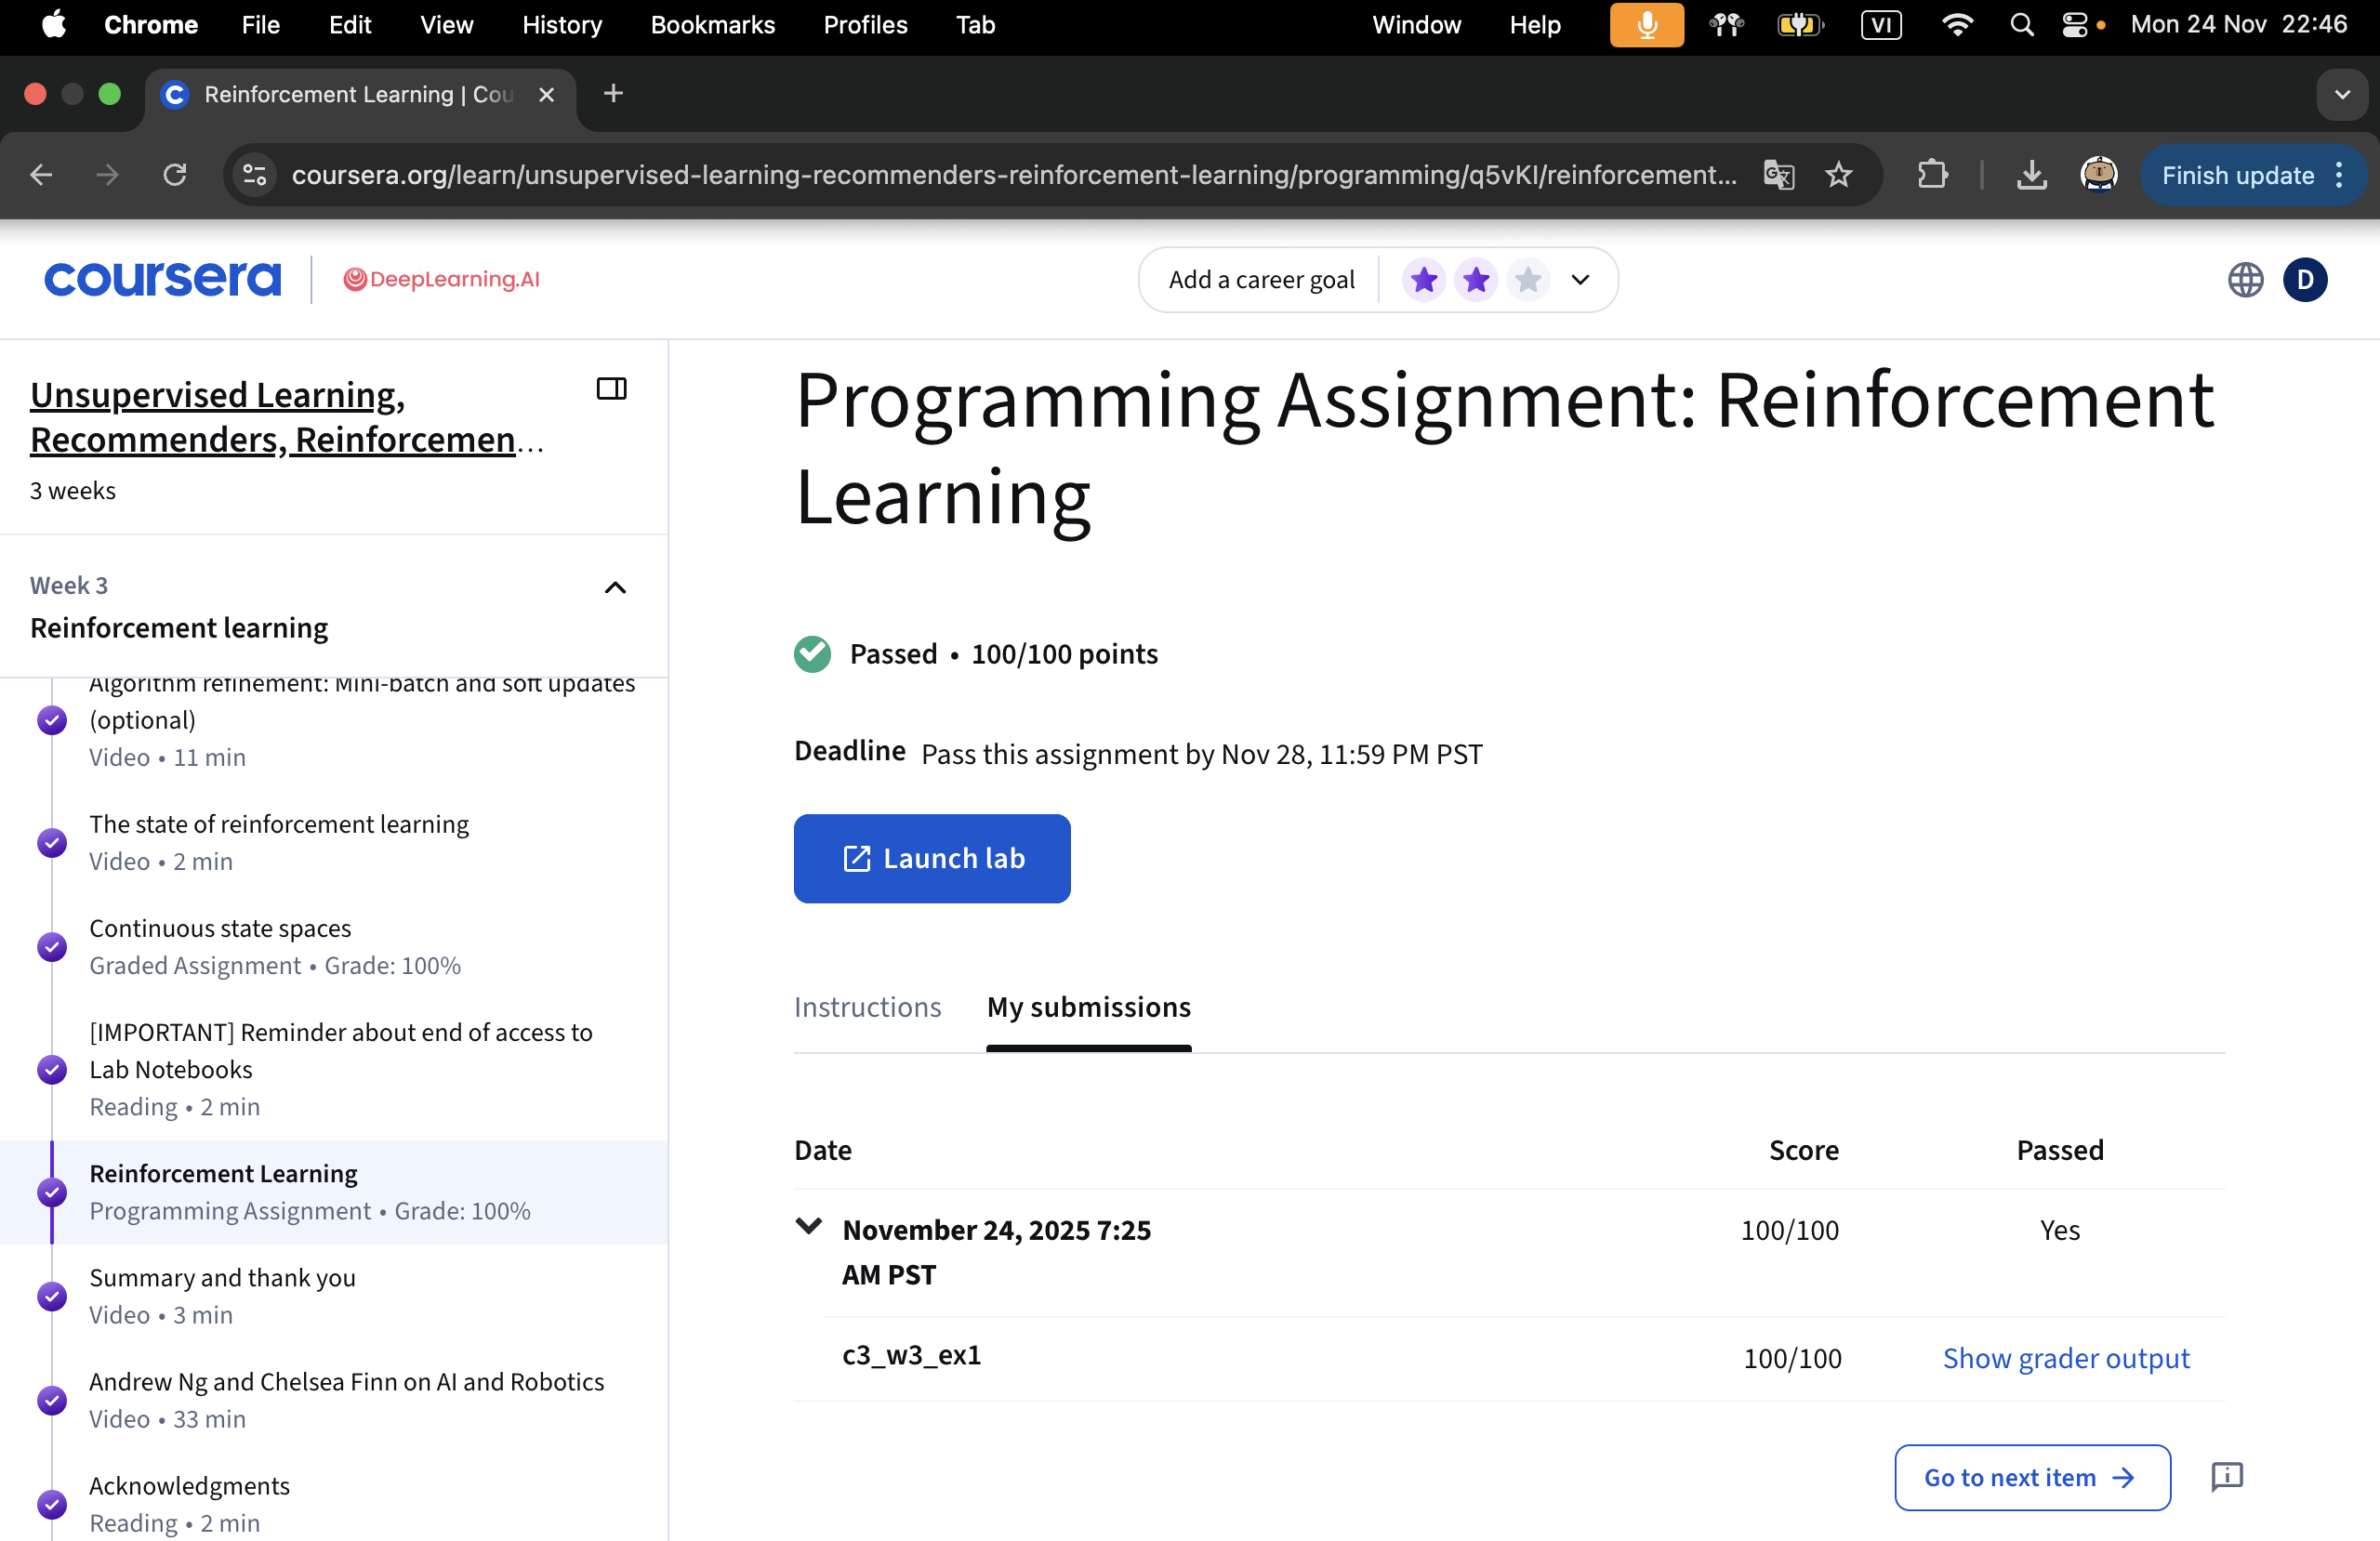
\includegraphics[scale=0.25]{Image/c3_w3_q4.png}
    \caption{Completed Programming Assignment (Reinforcement Learning)}
\end{figure}

\subsection{Certificate for Completion}
\begin{figure}[H]
    \centering
    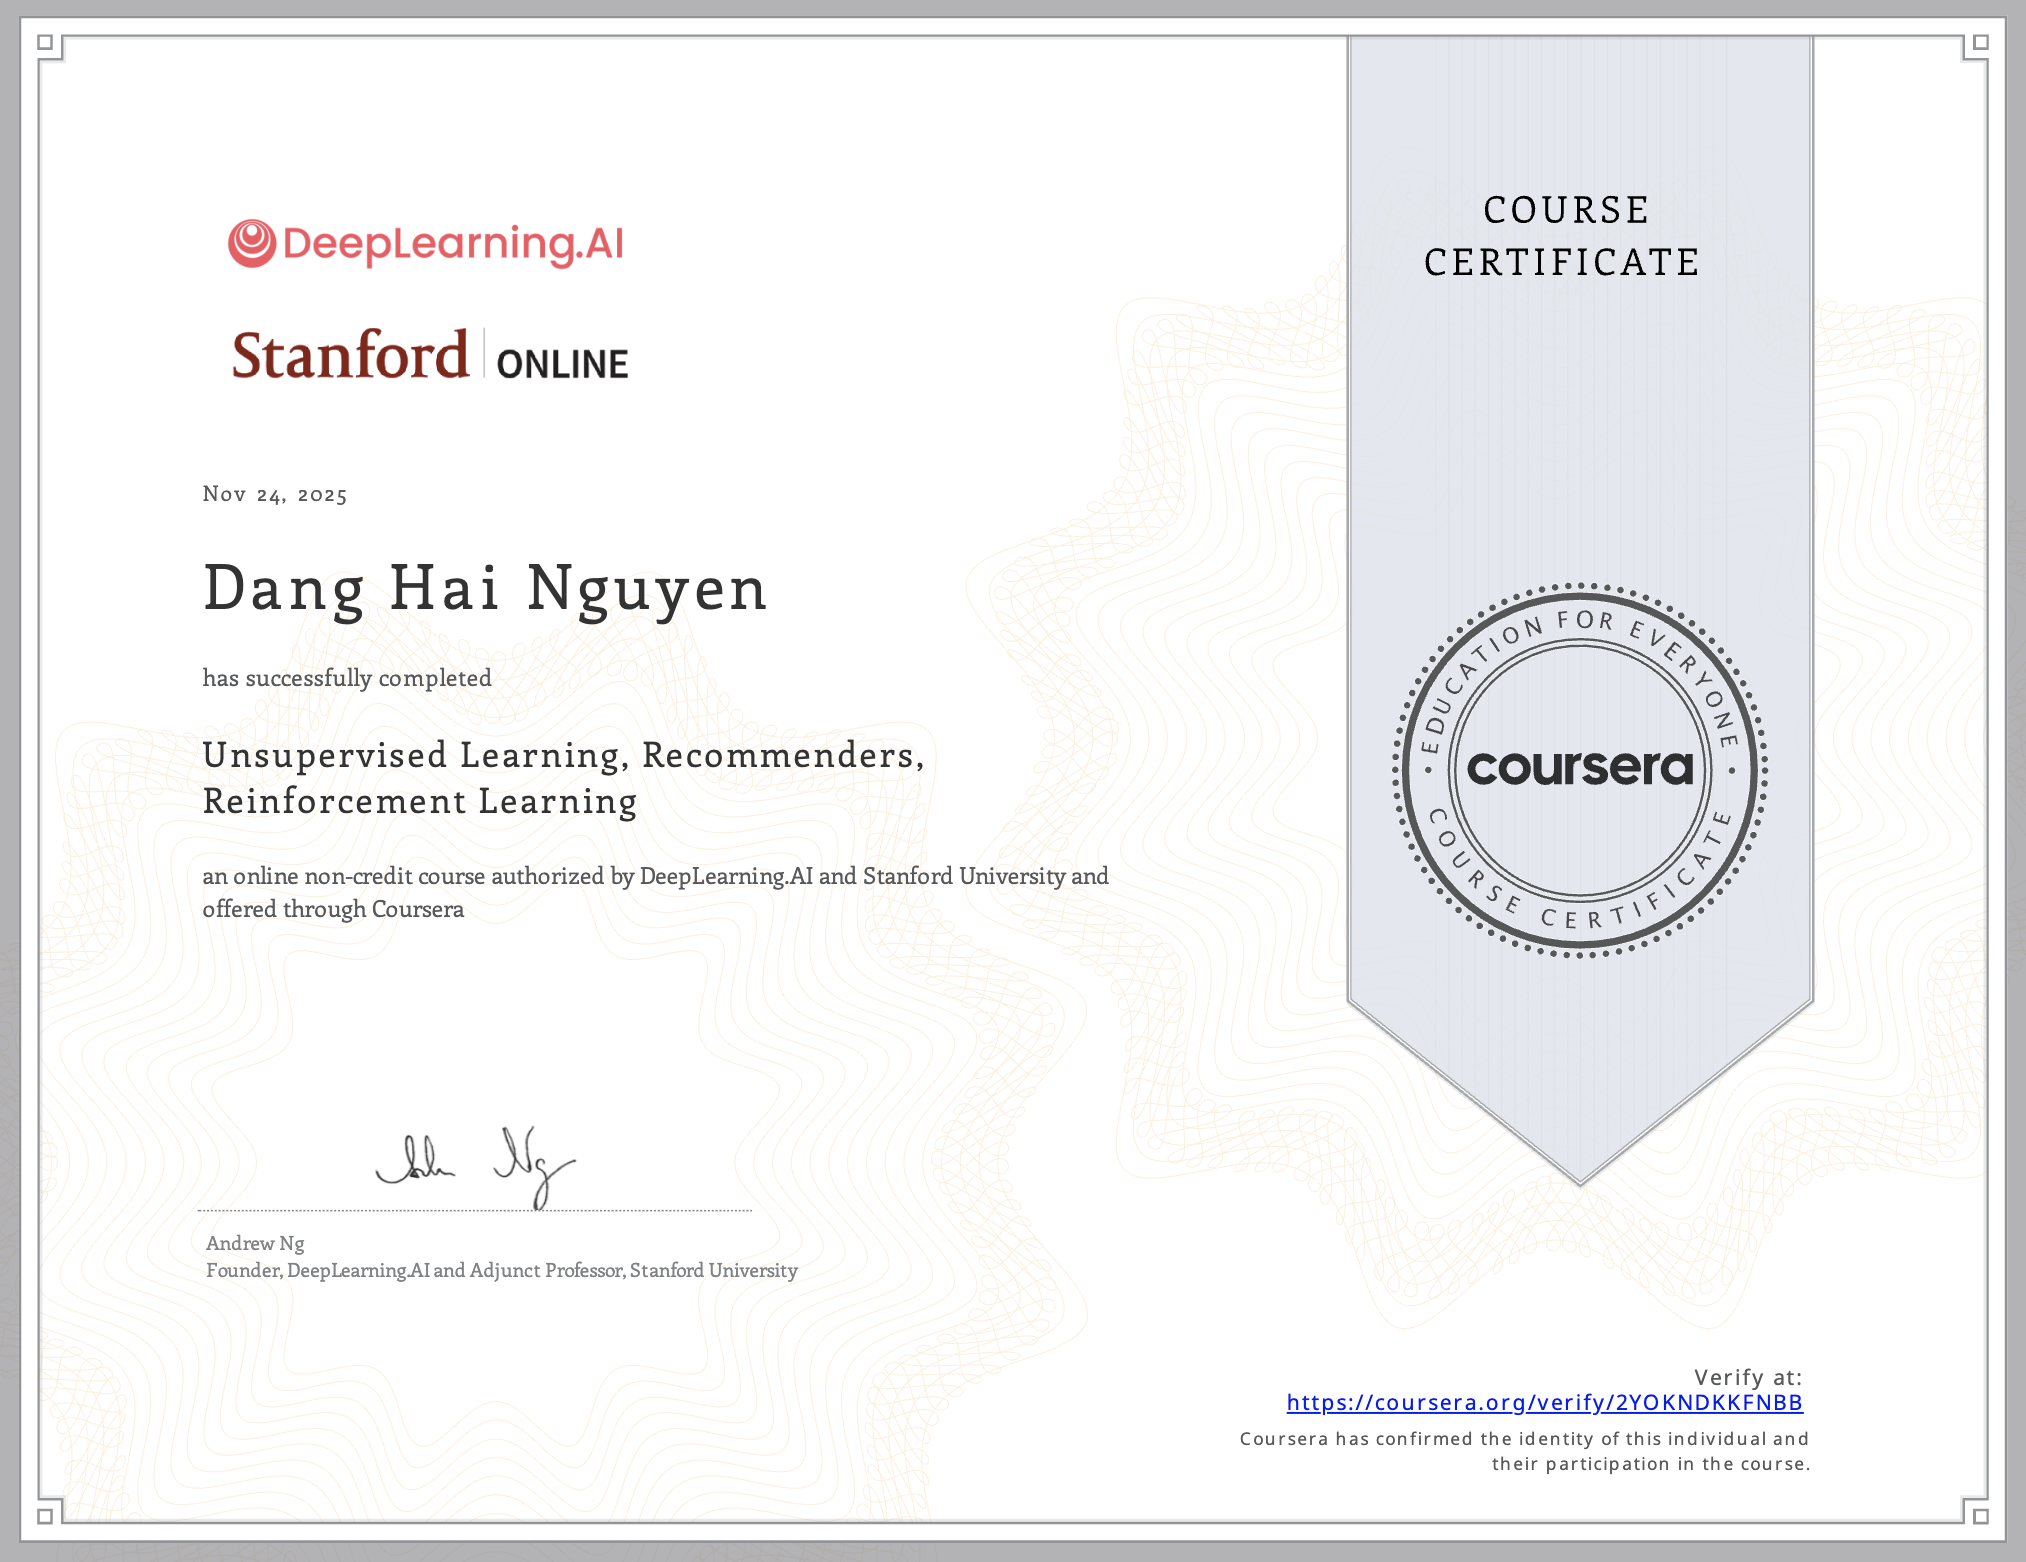
\includegraphics[scale=0.35]{Image/c3_certi.png}
    \caption{Certificate of completion for the course \textit{Unsupervised Learning, Recommenders, and Reinforcement Learning}.}
\end{figure}


